\documentclass[aspectratio=169]{beamer}
%[handout]

\usetheme[progressbar=frametitle]{metropolis}
\usepackage{appendixnumberbeamer}

\usepackage[utf8]{inputenc}
\usepackage[T1]{fontenc}

\usepackage[brazil]{babel}
\usepackage[outputdir=..]{minted}
\usepackage{xcolor}
\usepackage{soul} % strikethrough
\usepackage{advdate}
\usepackage{graphicx}
\graphicspath{{figs/}}
\usepackage{graphbox}

\usepackage[ampersand]{easylist}

\usepackage{multirow}
\usepackage{multicol}
\usepackage{subcaption}

\usepackage{pgf,tikz}
\usetikzlibrary{shapes,arrows,positioning}
\usetikzlibrary{circuits.logic.US}
\usetikzlibrary{matrix,calc}

\usepackage{karnaugh-map}

\usepackage{pgfpages}
\setbeameroption{hide notes} % Only slides
% \setbeameroption{show only notes} % Only notes
% \setbeameroption{show notes on second screen=right} % Both

% \graphicspath{{../figs/}}

\definecolor{bgc}{rgb}{0.95,0.9,0.95}
\definecolor{links}{HTML}{2A7F7F}
\hypersetup{colorlinks,linkcolor=,urlcolor=links}

\newminted{verilog}{fontsize=\scriptsize, 
    linenos,
    numbersep=8pt,
    bgcolor=bgc,
    tabsize=4,
    framesep=3mm} 
    %frame=lines,

\newcommand{\verilog}[1]{\verilogf{#1}{\footnotesize}}

\newcommand{\verilogf}[2]{\inputminted[fontsize=#2, 
    linenos,
    tabsize=2,
    numbersep=4pt,
    bgcolor=bgc,
    framesep=3mm]{verilog}{../codes/#1.v}
}

\newminted{nasm}{fontsize=\scriptsize, 
		   linenos,
		   numbersep=8pt,
           bgcolor=bgc,
		   framesep=3mm} 

\usepackage{booktabs}
\usepackage[scale=2]{ccicons}

\usepackage{pgfplots}
\usepgfplotslibrary{dateplot}

\usepackage{hyperref}


\usepackage{xspace}
\newcommand{\themename}{\textbf{\textsc{metropolis}}\xspace}



\usepackage{pifont}% http://ctan.org/pkg/pifont
\newcommand{\cmark}{\ding{51}}%
\newcommand{\xmark}{\ding{55}}%

% \tiny	
% \scriptsize
% \footnotesize
% \small	
% \normalsize	
% \large	
% \Large	
% \LARGE	
% \huge	
% \Huge	



\newminted{python}{fontsize=\scriptsize, 
		   linenos,
		   breaklines,
		   numbersep=8pt,
           tabsize=2,
		   framesep=3mm} 
		   
\newminted{verilog}{fontsize=\scriptsize, 
		   linenos,
		   breaklines,
		   numbersep=8pt,
           tabsize=2,
		   framesep=3mm} 
		   




\definecolor{bgc}{rgb}{0.95,0.9,0.95}
\definecolor{links}{HTML}{2A7F7F}
\hypersetup{colorlinks,linkcolor=,urlcolor=links}


% \usepackage[style=apa]{biblatex}
% \addbibresource{mm.bib}


% \author{\large Prof. Ricardo Menotti (\href{mailto:menotti@ufscar.br}{menotti@ufscar.br})}

\newcommand{\newauthor}[2]{
  \parbox{0.50\textwidth}{
    \texorpdfstring
      {
        \centering
        \small #1 \newline
        {\scriptsize{\urlstyle{same}\href{mailto:#2}{#2}\urlstyle{tt}}}
      }
      {#1} \newline
  }
}

\author{
  \newauthor{Prof. Ricardo Menotti}{menotti@ufscar.br}
\and \newauthor{Prof. Luciano de Oliveira Neris}{lneris@ufscar.br}  
%\and \newauthor{Prof. Artino Quintino da Silva Filho}{artino@ufscar.br}
% \and \newauthor{Prof. Maurício Figueiredo}{mauricio@ufscar.br}
% \and \newauthor{Prof. Edilson Kato}{kato@ufscar.br}
% \and \newauthor{Prof. Roberto Inoue}{rsinoue@ufscar.br}
}

\date{Atualizado em: \today}

\institute{\large \textbf{Departamento de Computação} \\
Centro de Ciências Exatas e de Tecnologia \\
Universidade Federal de São Carlos}

\title{Lógica Digital (1001351)}

\titlegraphic{\hfill
\includegraphics[height=1.5cm]{LogoUfscar}}



\subtitle{Representação Numérica e Circuitos Aritméticos} % 

\begin{document}

\begin{frame}
	\titlepage
\end{frame} 

%%%%%%%%%%%%%%%%%%%%%%%%%%%%%%%%%%%%%%%%%%%%%%%%%%%%%%%%%%%%%%%%%%%%%%%%%%%%%%%%

\section{Relembrando...}

\begin{frame}{\insertsection}
	\begin{itemize}
        \item No sistema numérico binário, é usada a representação numérica posicional:
        \begin{itemize}
            \item $B = b_{n-1}b_{n-2} ... b_1 b_0$
            \item $V(B) = b_{n-1} \times 2^{n-1} + b_{n-2} \times 2^{n-2} ... b_1 \times 2^1 + b_0 \times 2^0$
            \item $= \sum\limits_{i=0}^{n-1} b_i \times 2^i$
        \end{itemize}
    \end{itemize}
    \center 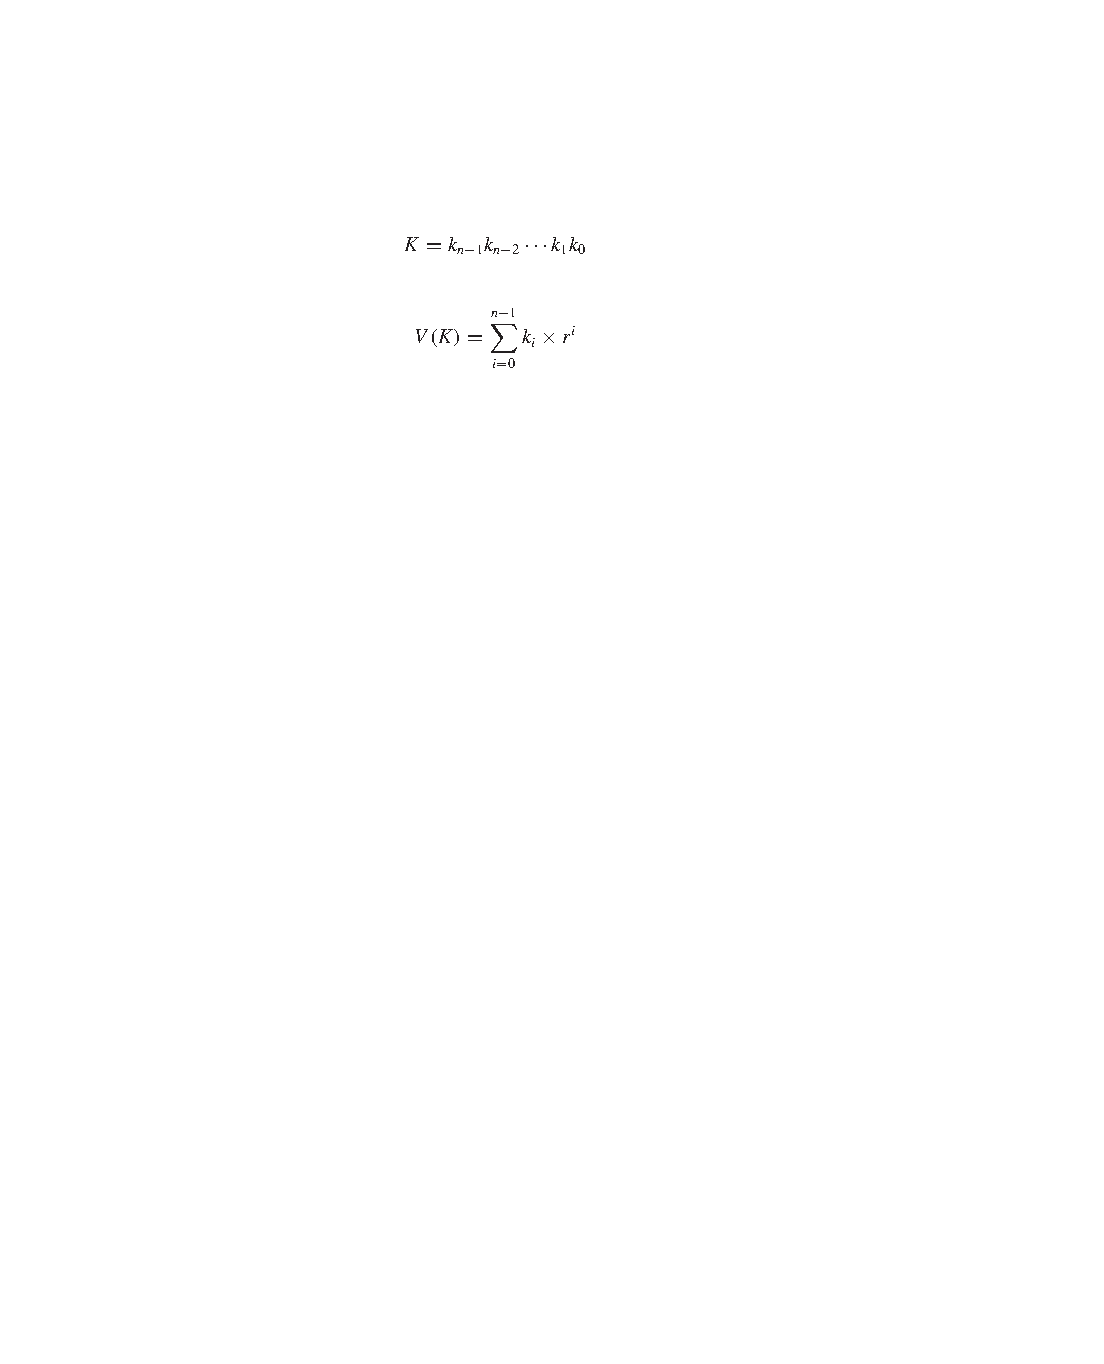
\includegraphics[]{VerilogFig3_1_2}
\end{frame}

\section{Representações Octal e Hexadecimal}

\begin{frame}{\insertsection}
    \center 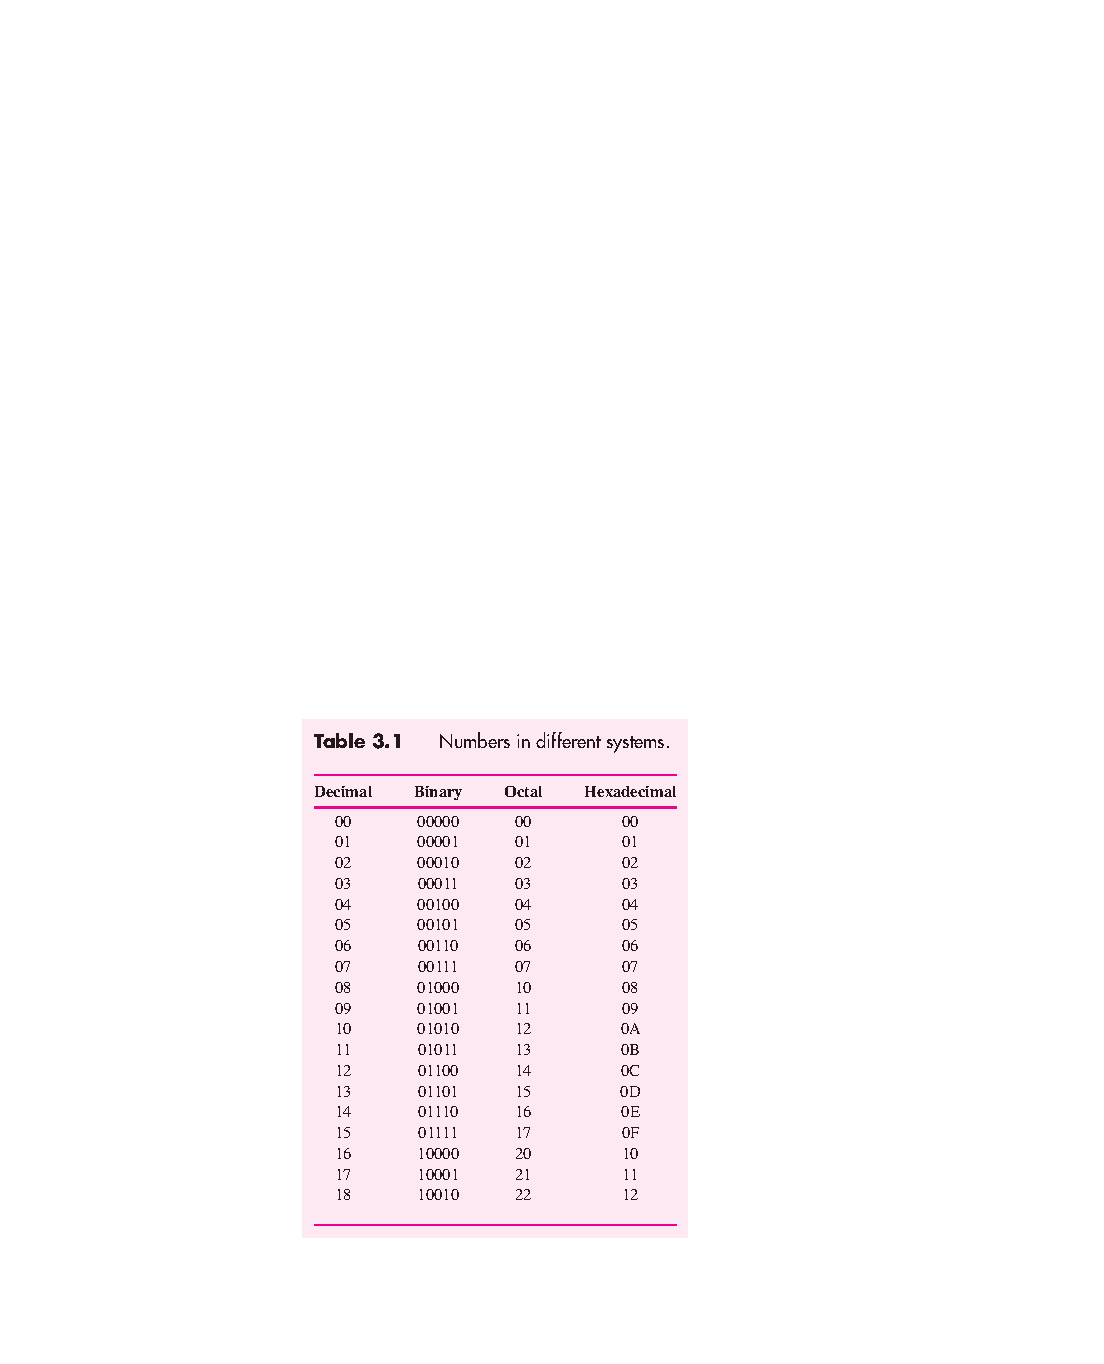
\includegraphics[scale=.85]{VerilogTab3_1}
\end{frame}

\begin{frame}{\insertsection}
    \center
    $101011010111_{(2)}=5327_{(8)}$ \\
    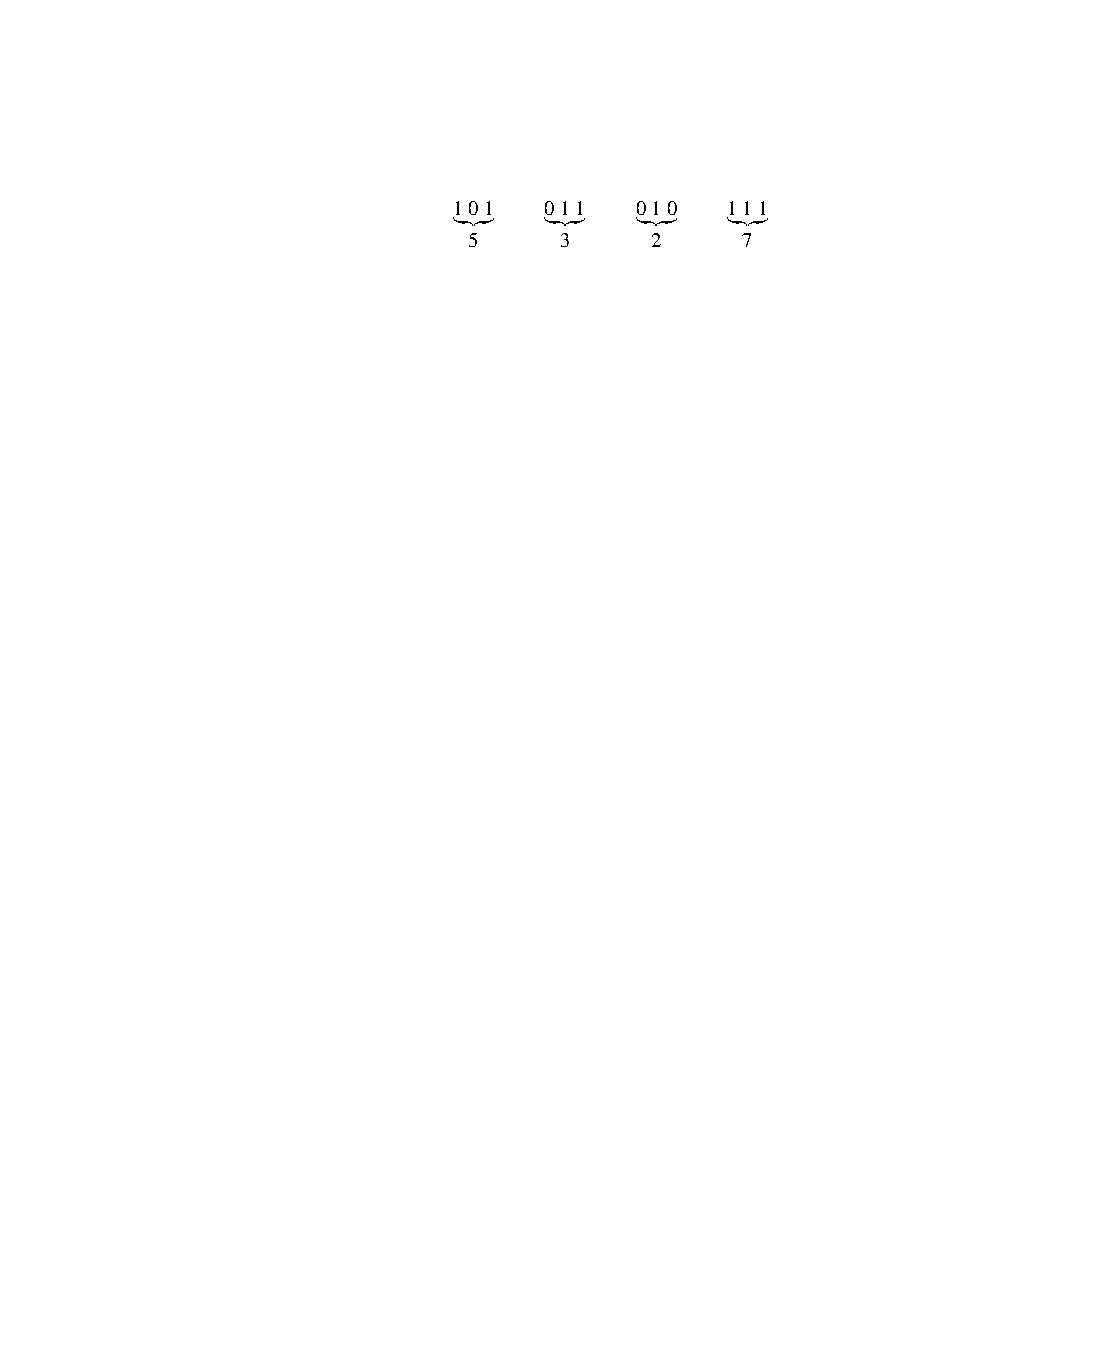
\includegraphics{Octal5327} \\
    \vspace{2cm}
    \pause
    $010111011_{(2)}=273_{(8)}$ \\
    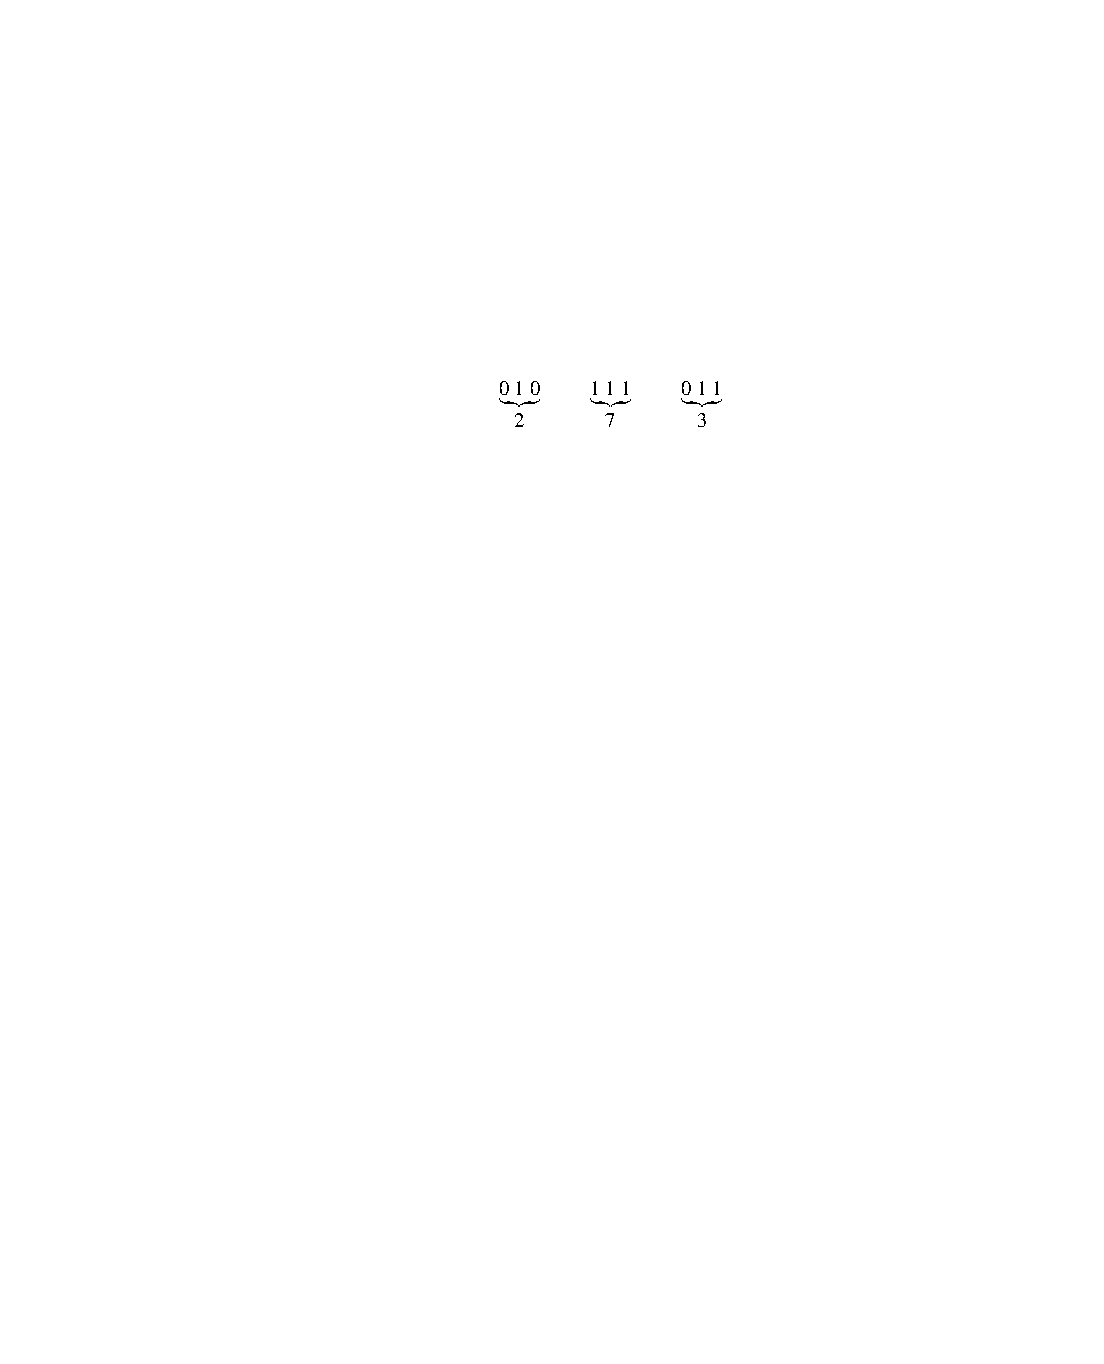
\includegraphics{Octal273} \\
\end{frame}

\begin{frame}{\insertsection}
    \center
    $1010111100100101_{(2)}=AF25_{(16)}$ \\
    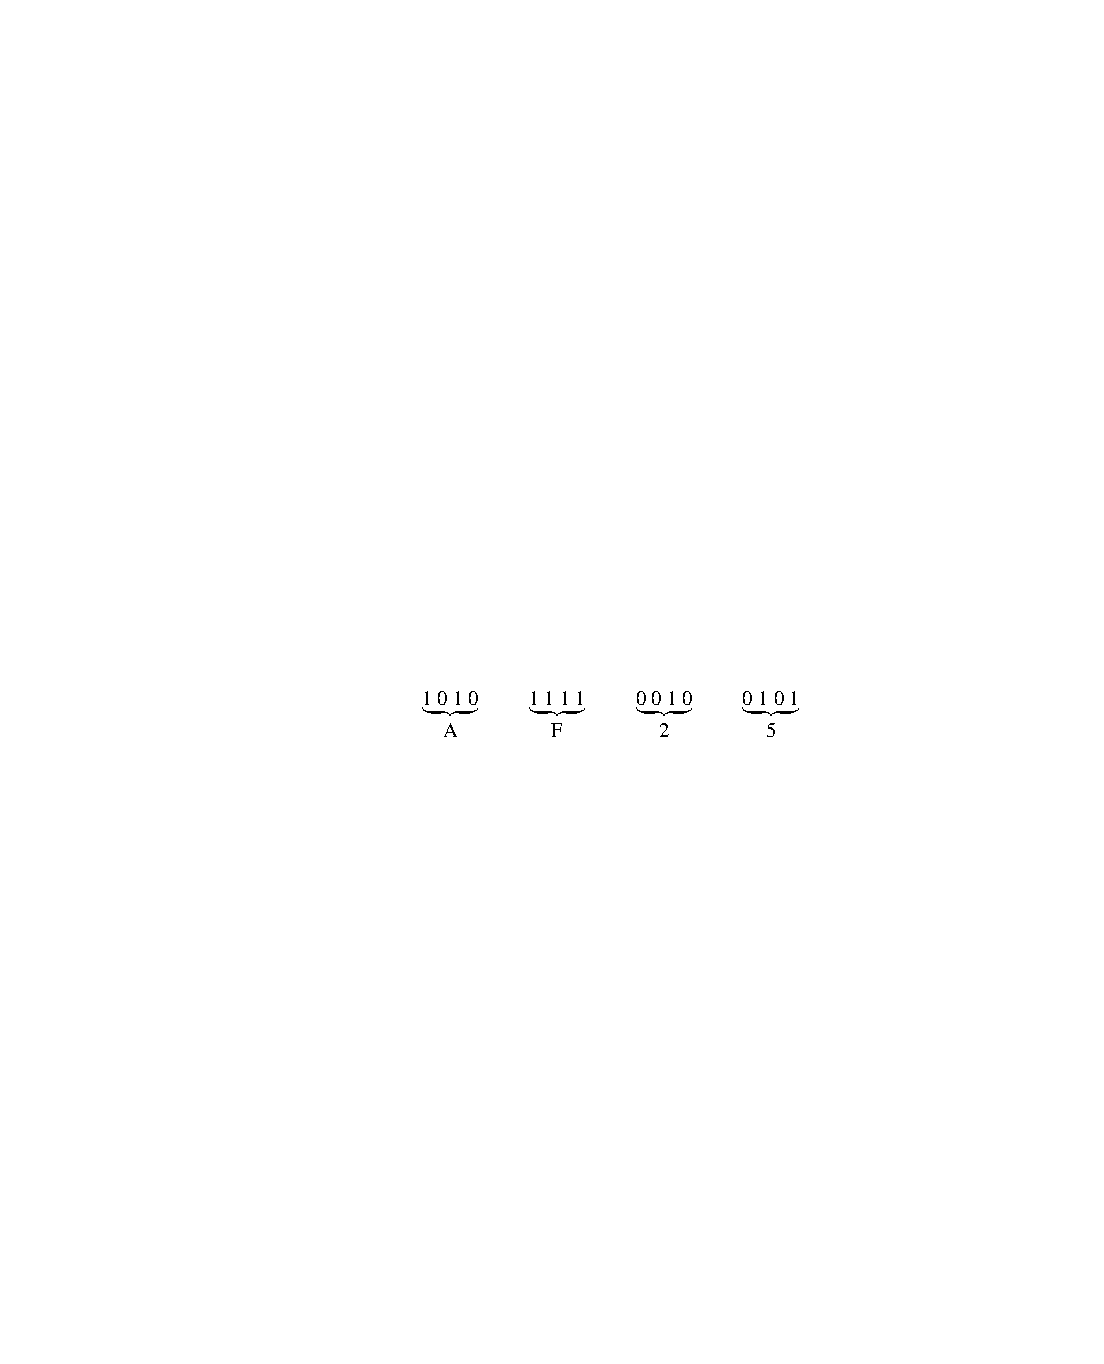
\includegraphics{HexaAF25} \\
    \pause
    \vspace{2cm}
    $001101101000_{(2)}=368_{(16)}=$ \\
    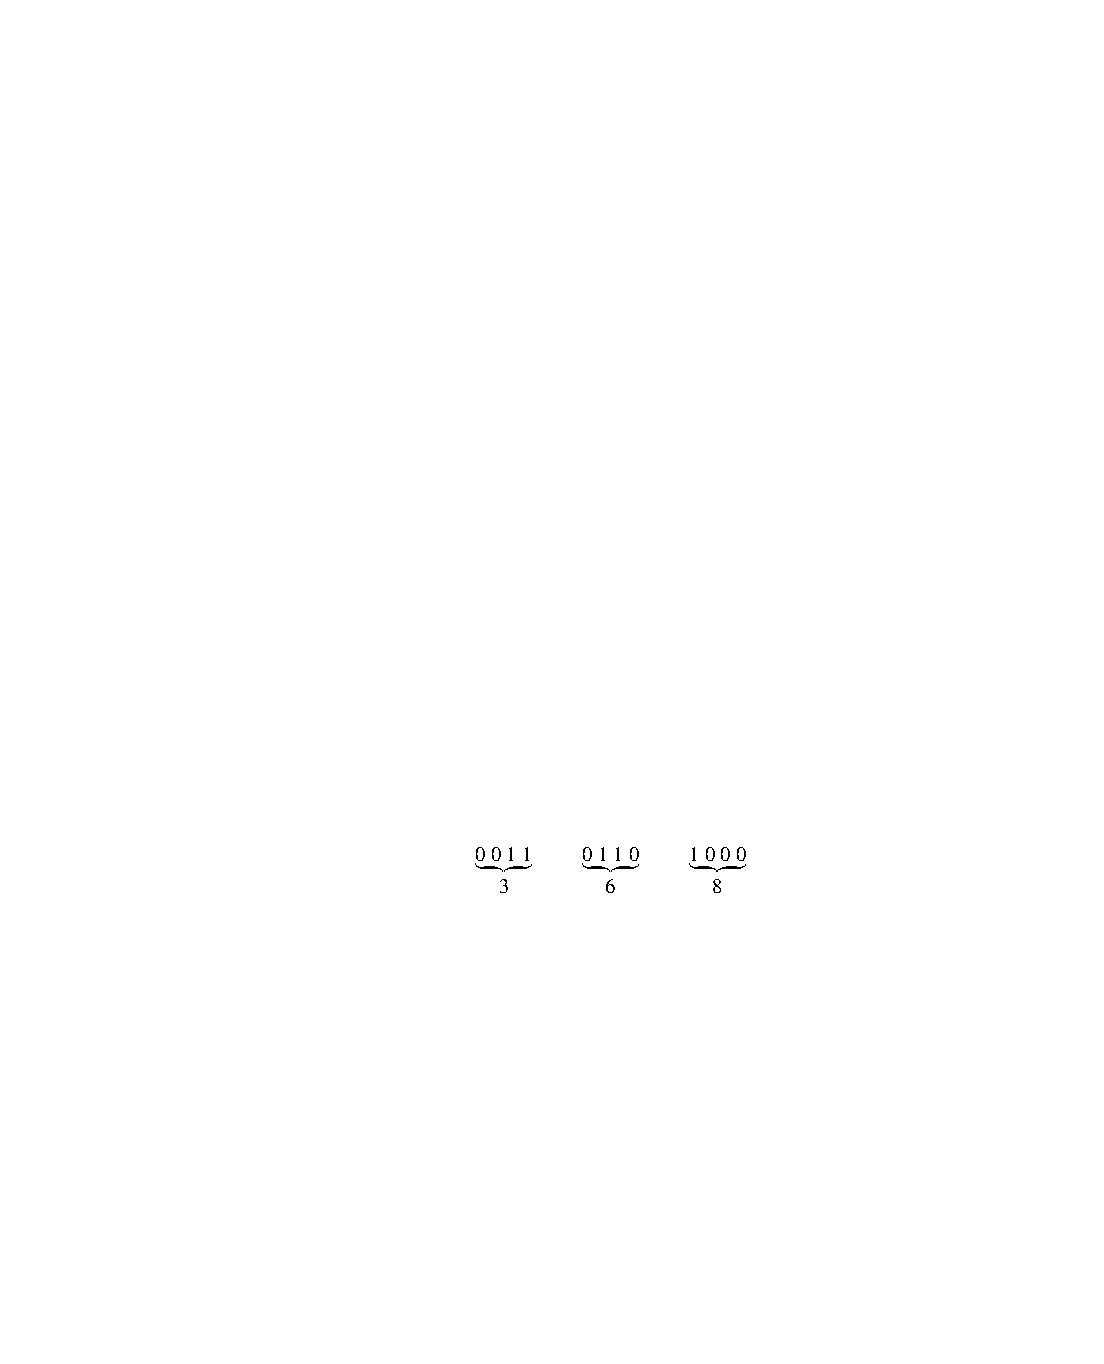
\includegraphics{Hexa368}
\end{frame}

\section{Adição de números sem sinal}

\begin{frame}{\insertsection}
    \begin{columns}
        \begin{column}{.6\textwidth}
            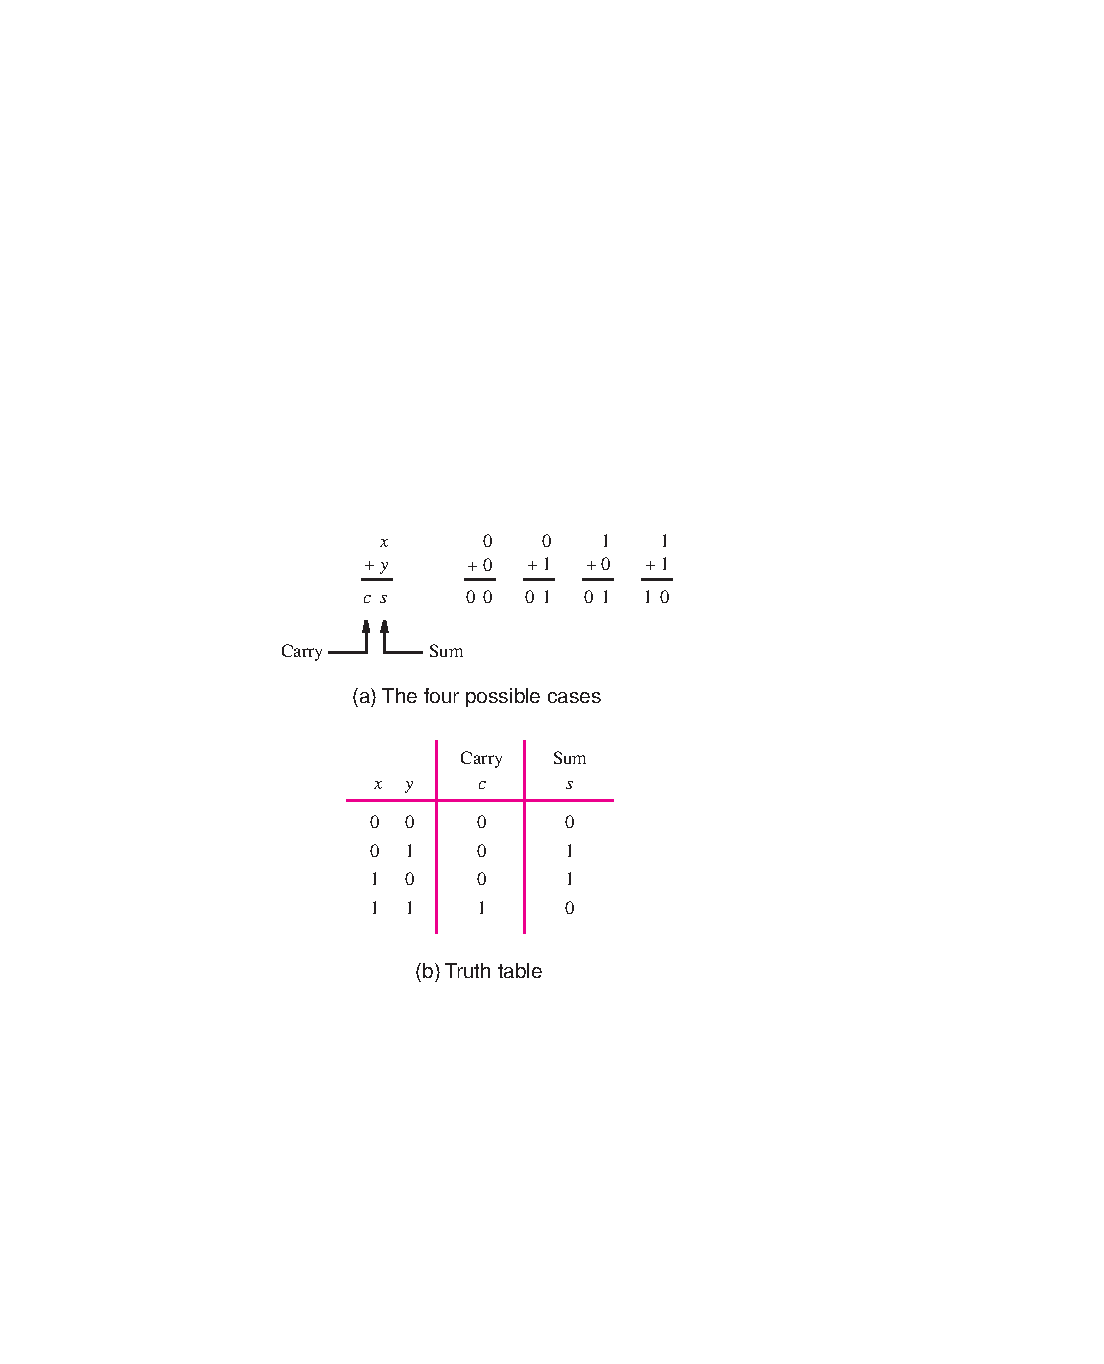
\includegraphics[width=.74\textwidth]{VerilogFig3_1ab}
        \end{column}
        \begin{column}{.4\textwidth}
            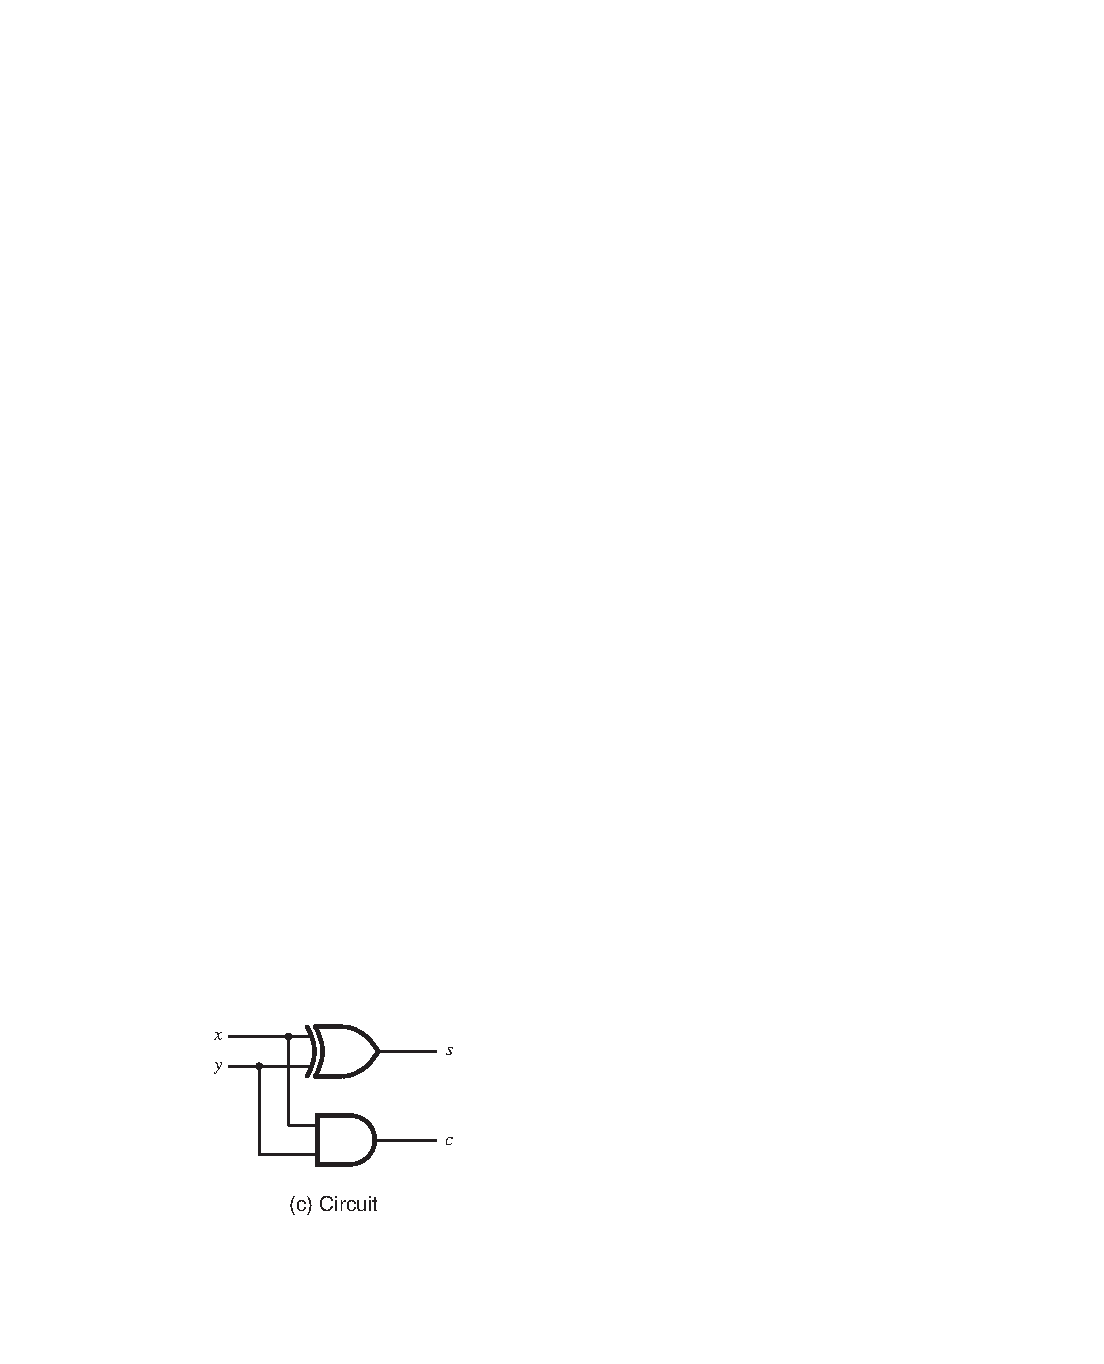
\includegraphics[width=.74\textwidth]{VerilogFig3_1c} \\
            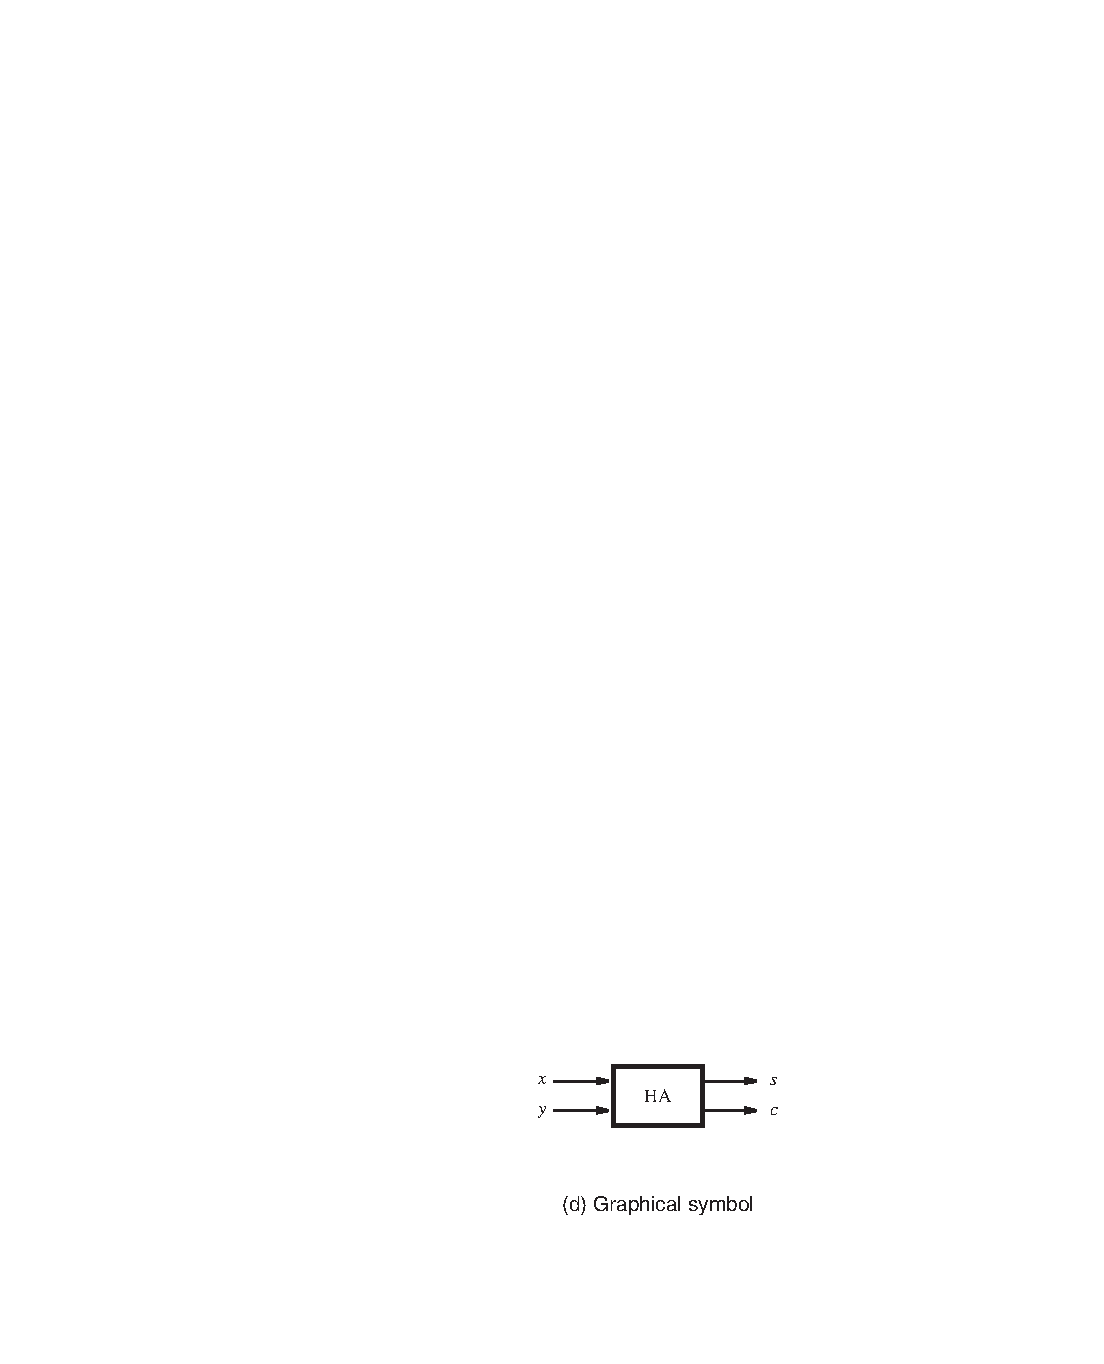
\includegraphics[width=.74\textwidth]{VerilogFig3_1d}
        \end{column}
    \end{columns}
    \center 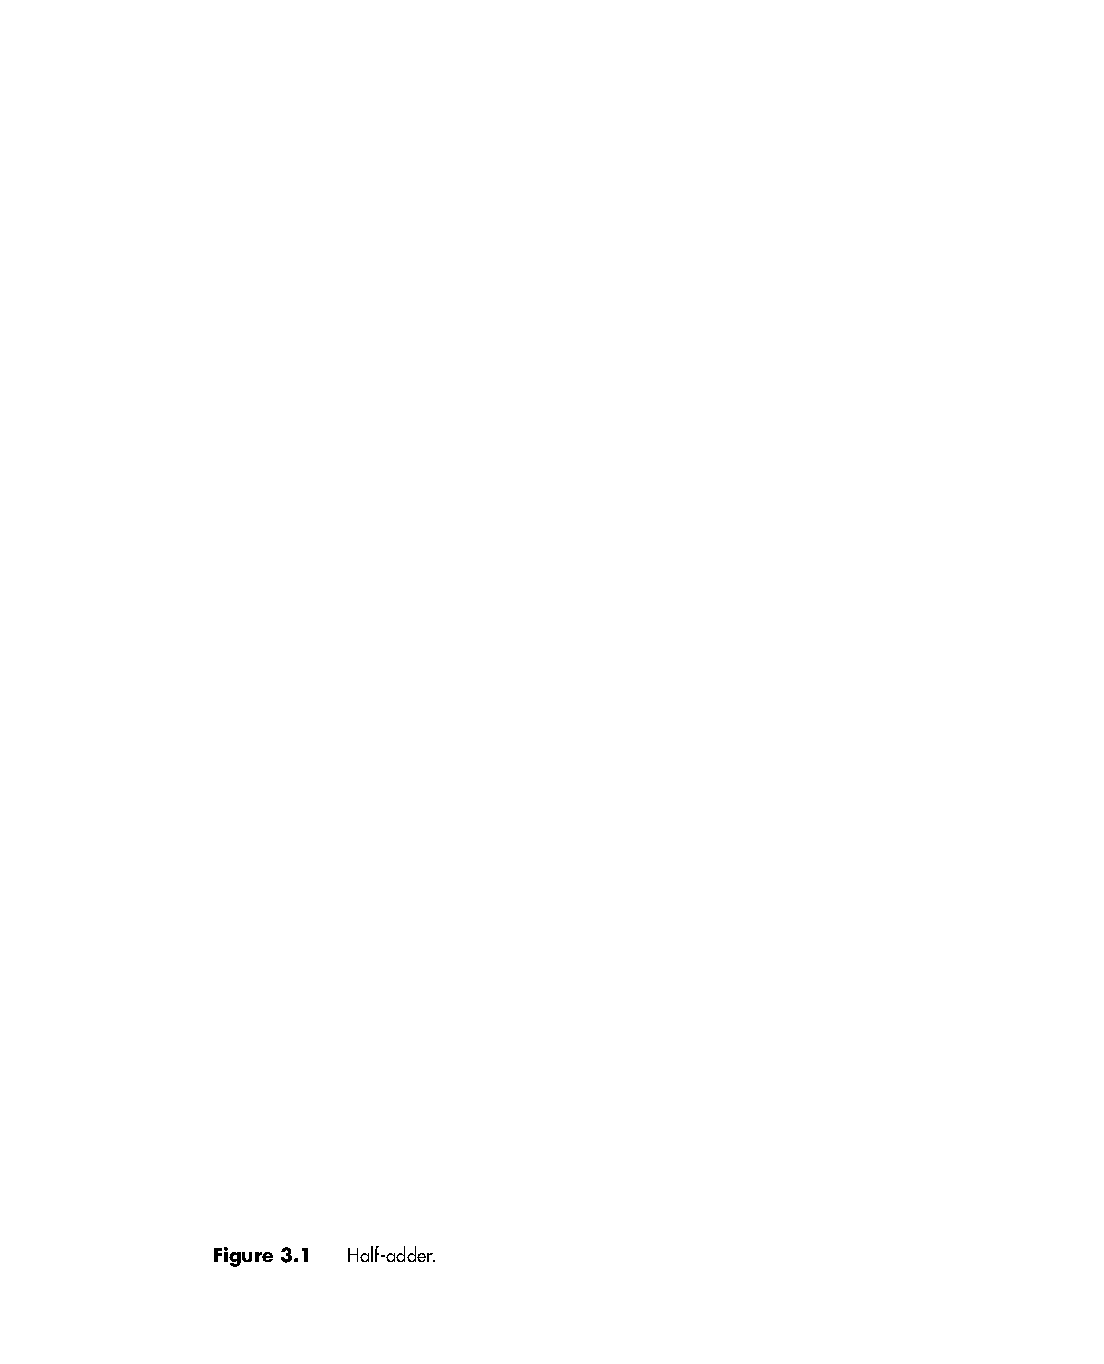
\includegraphics[]{VerilogFig3_1}
\end{frame}

\begin{frame}{\insertsection}
    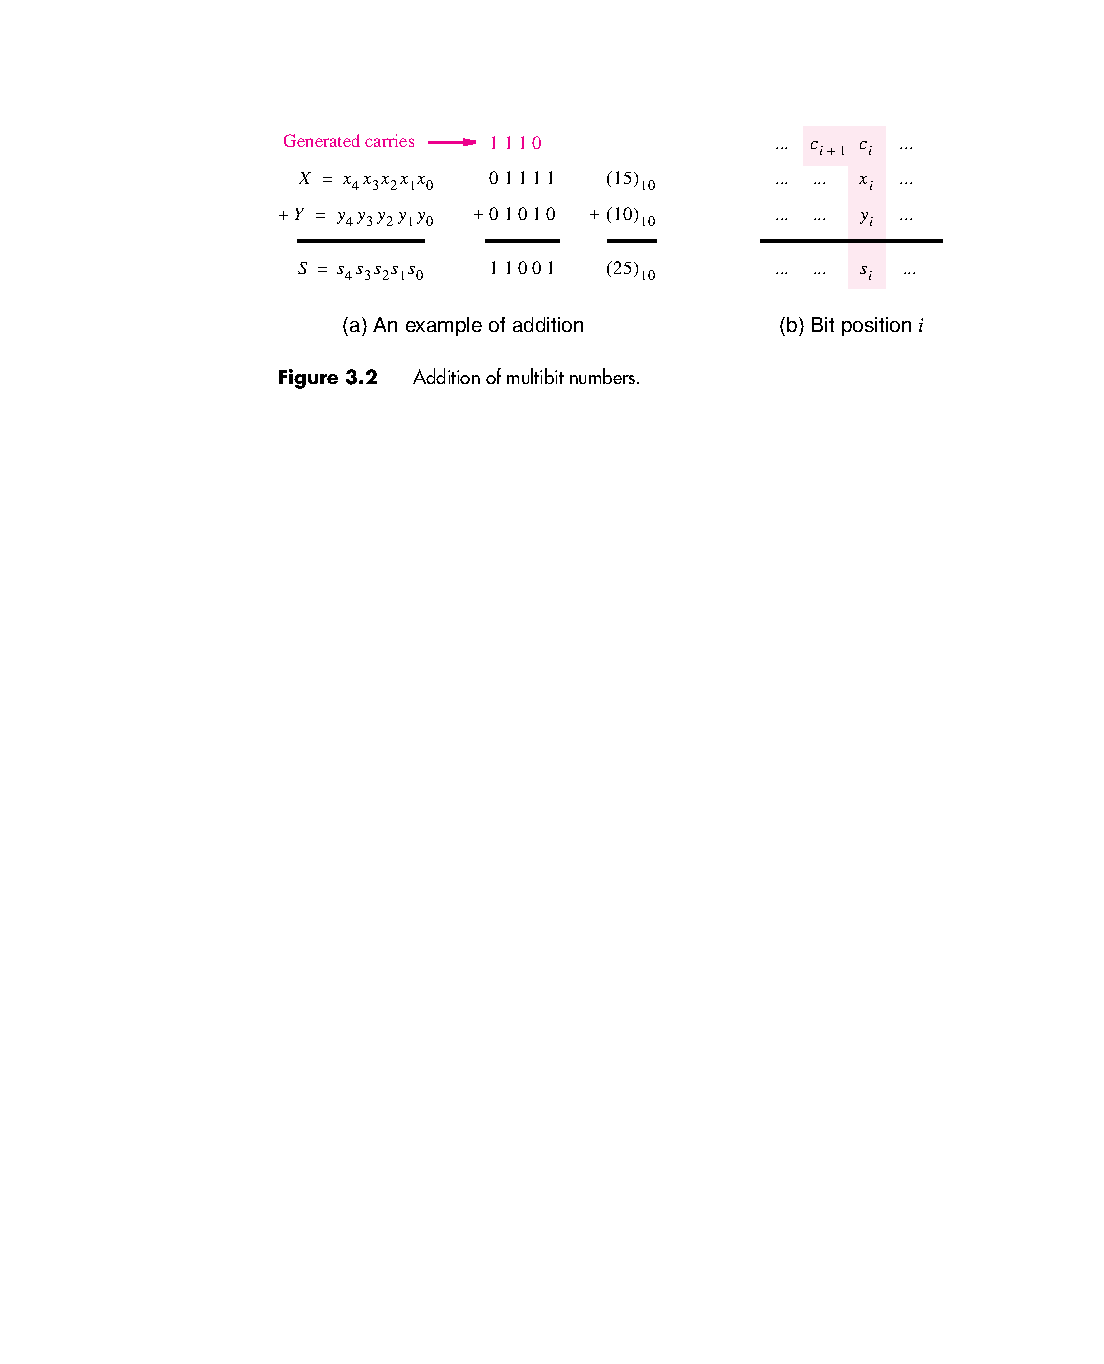
\includegraphics[width=\textwidth]{VerilogFig3_2}
\end{frame}

\begin{frame}{\insertsection}
    \begin{columns}
        \begin{column}{.35\textwidth}
            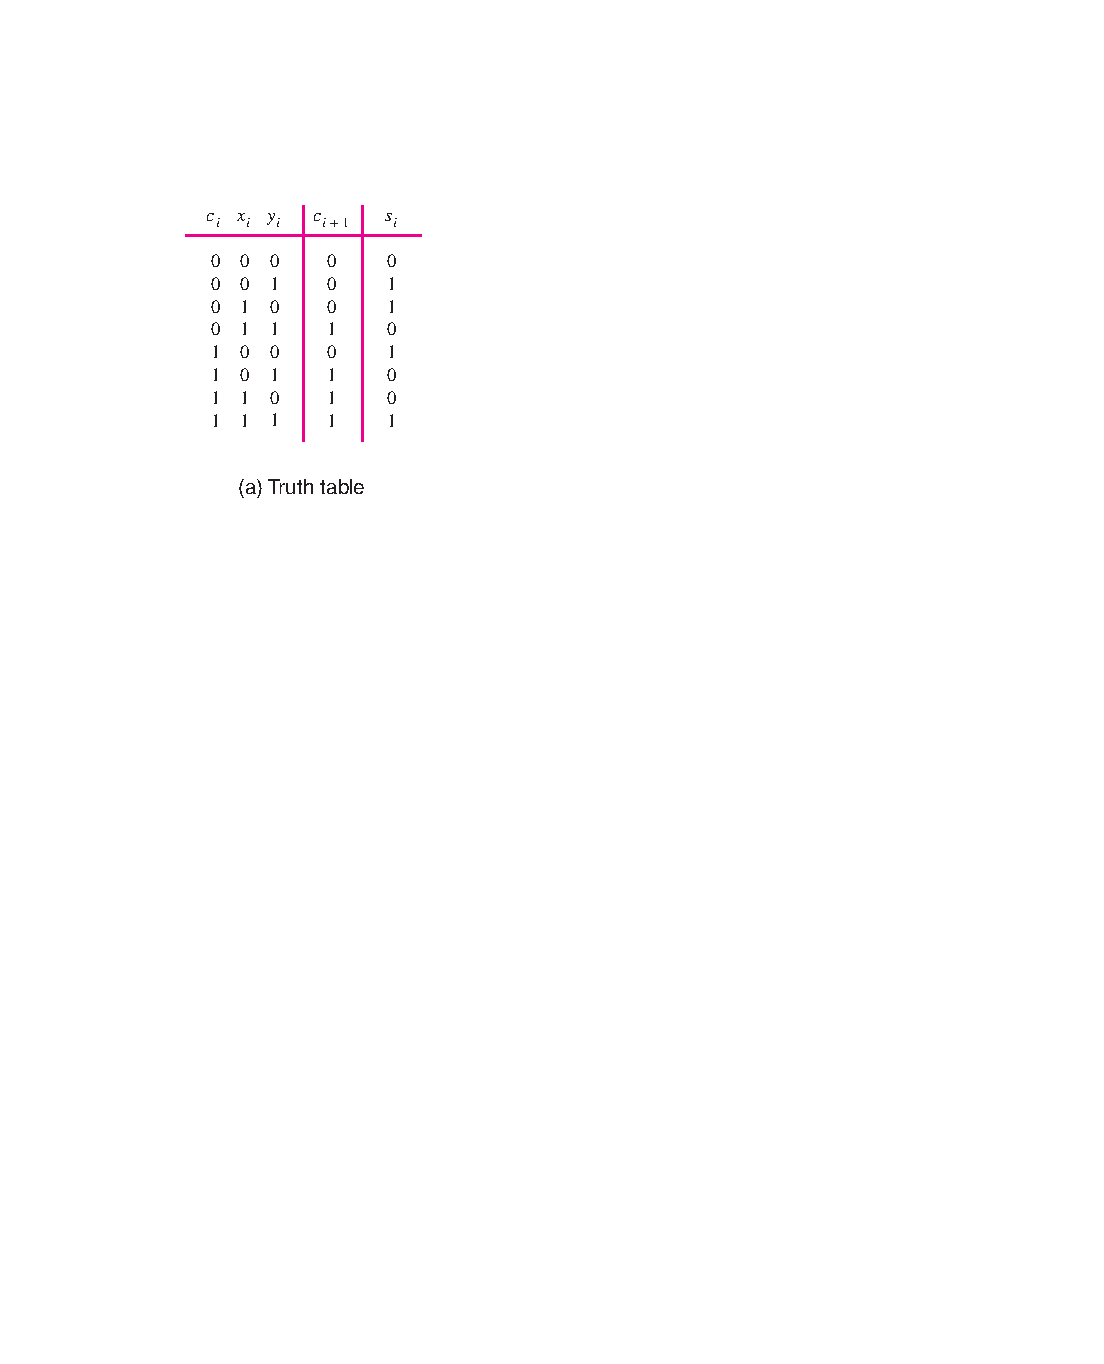
\includegraphics[width=.55\textwidth]{VerilogFig3_3a} \\
            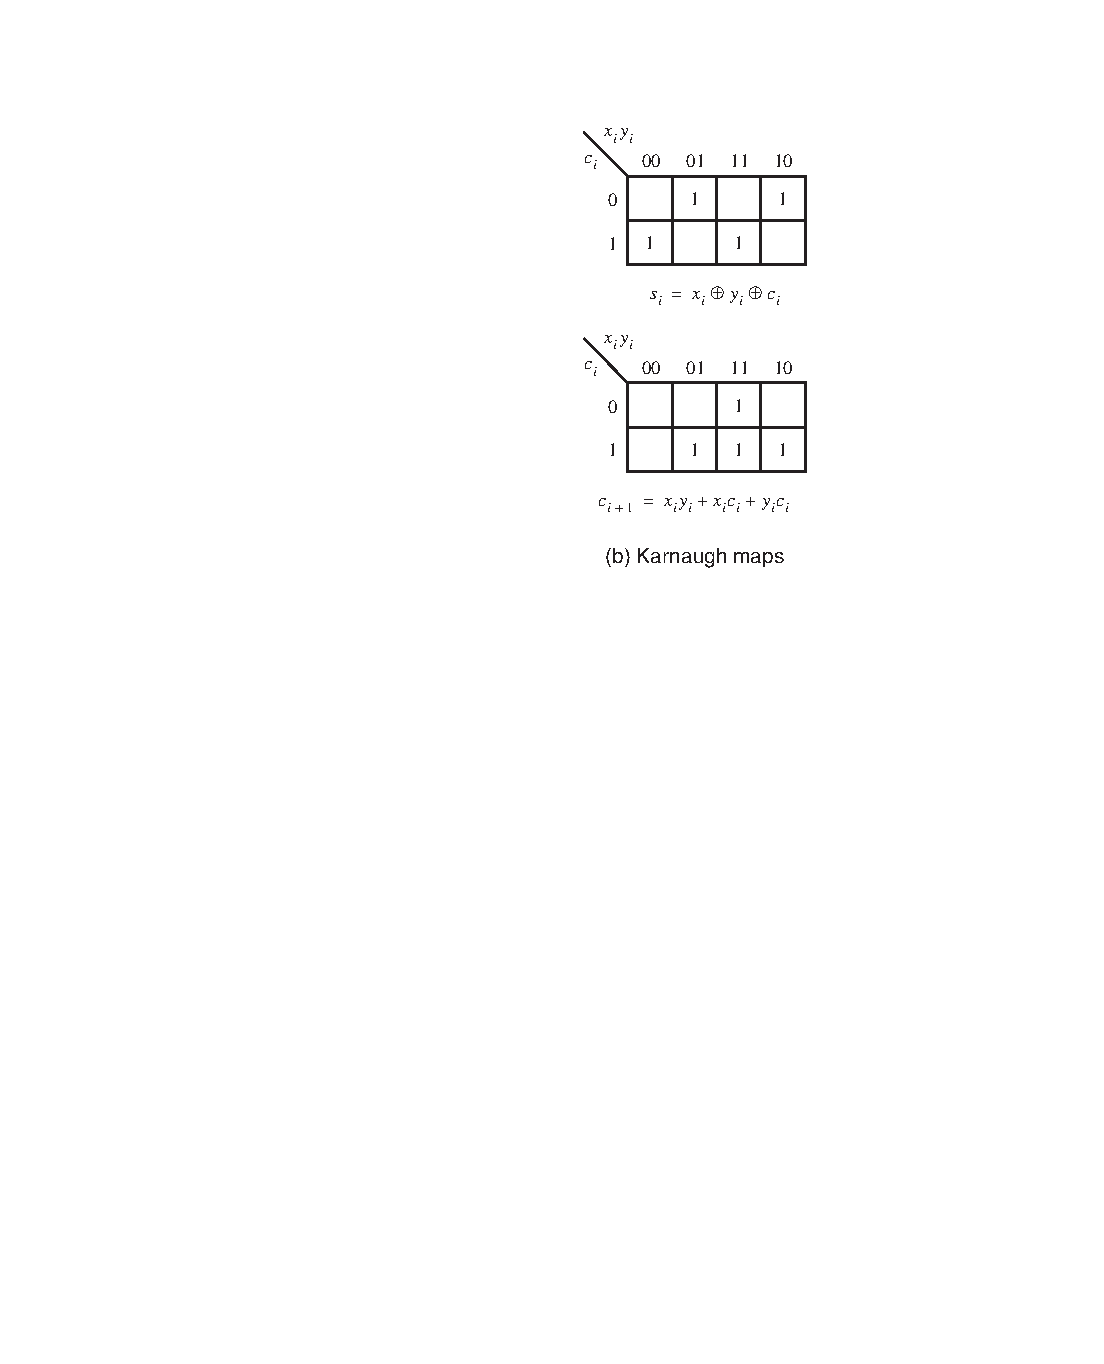
\includegraphics[width=.55\textwidth]{VerilogFig3_3b}
        \end{column}
        \begin{column}{.55\textwidth}
            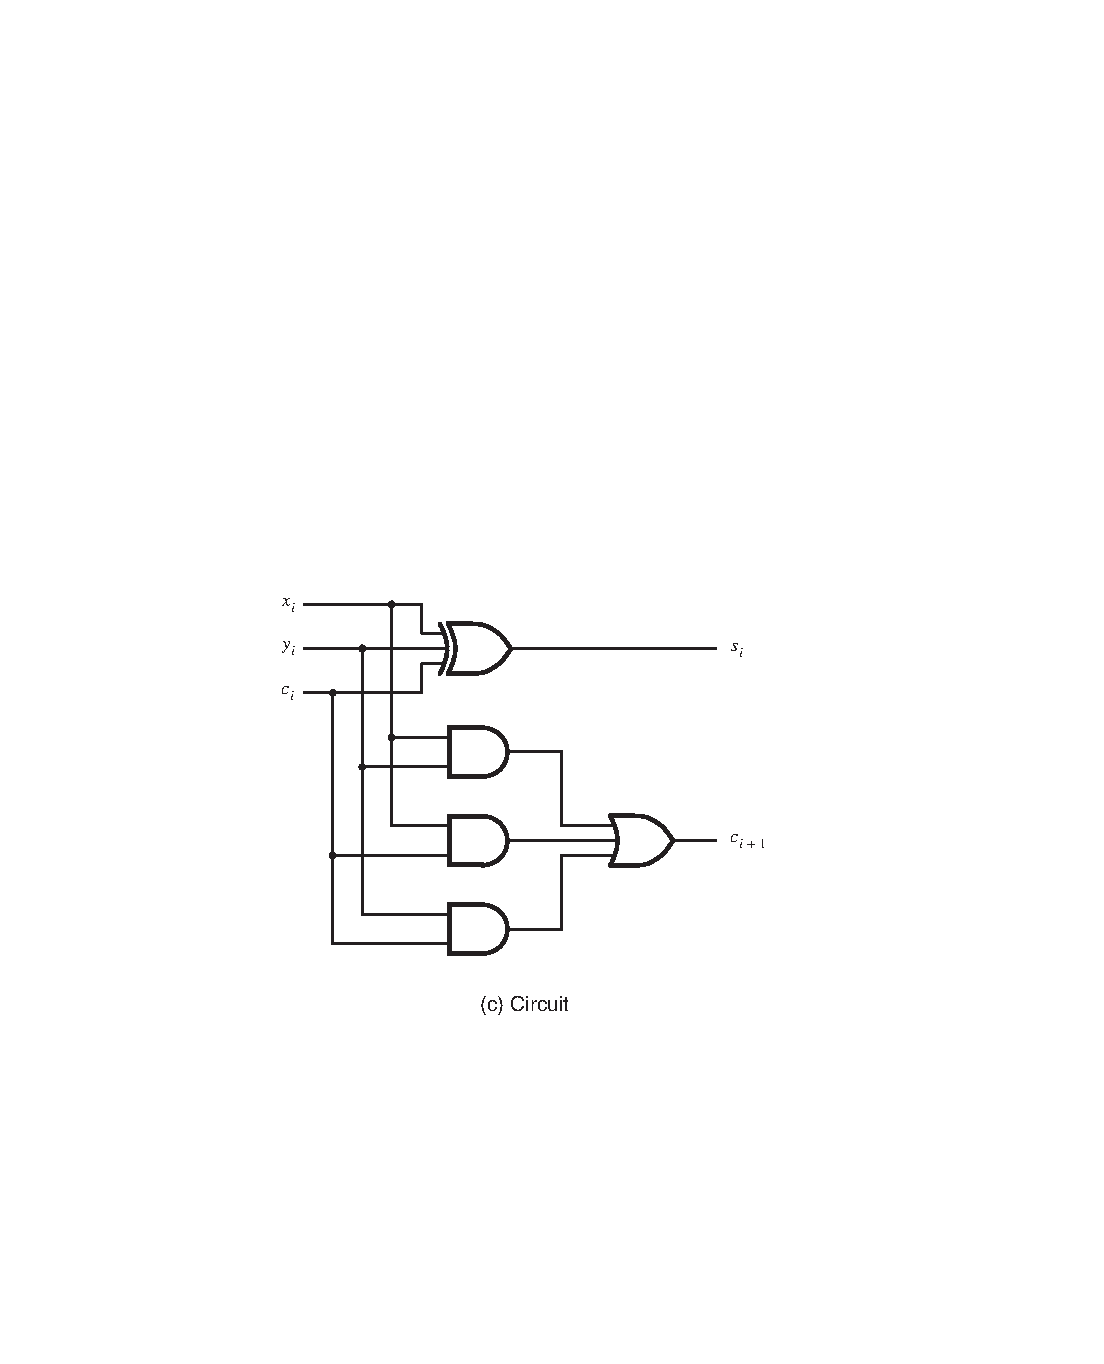
\includegraphics[width=\textwidth]{VerilogFig3_3c} \\
            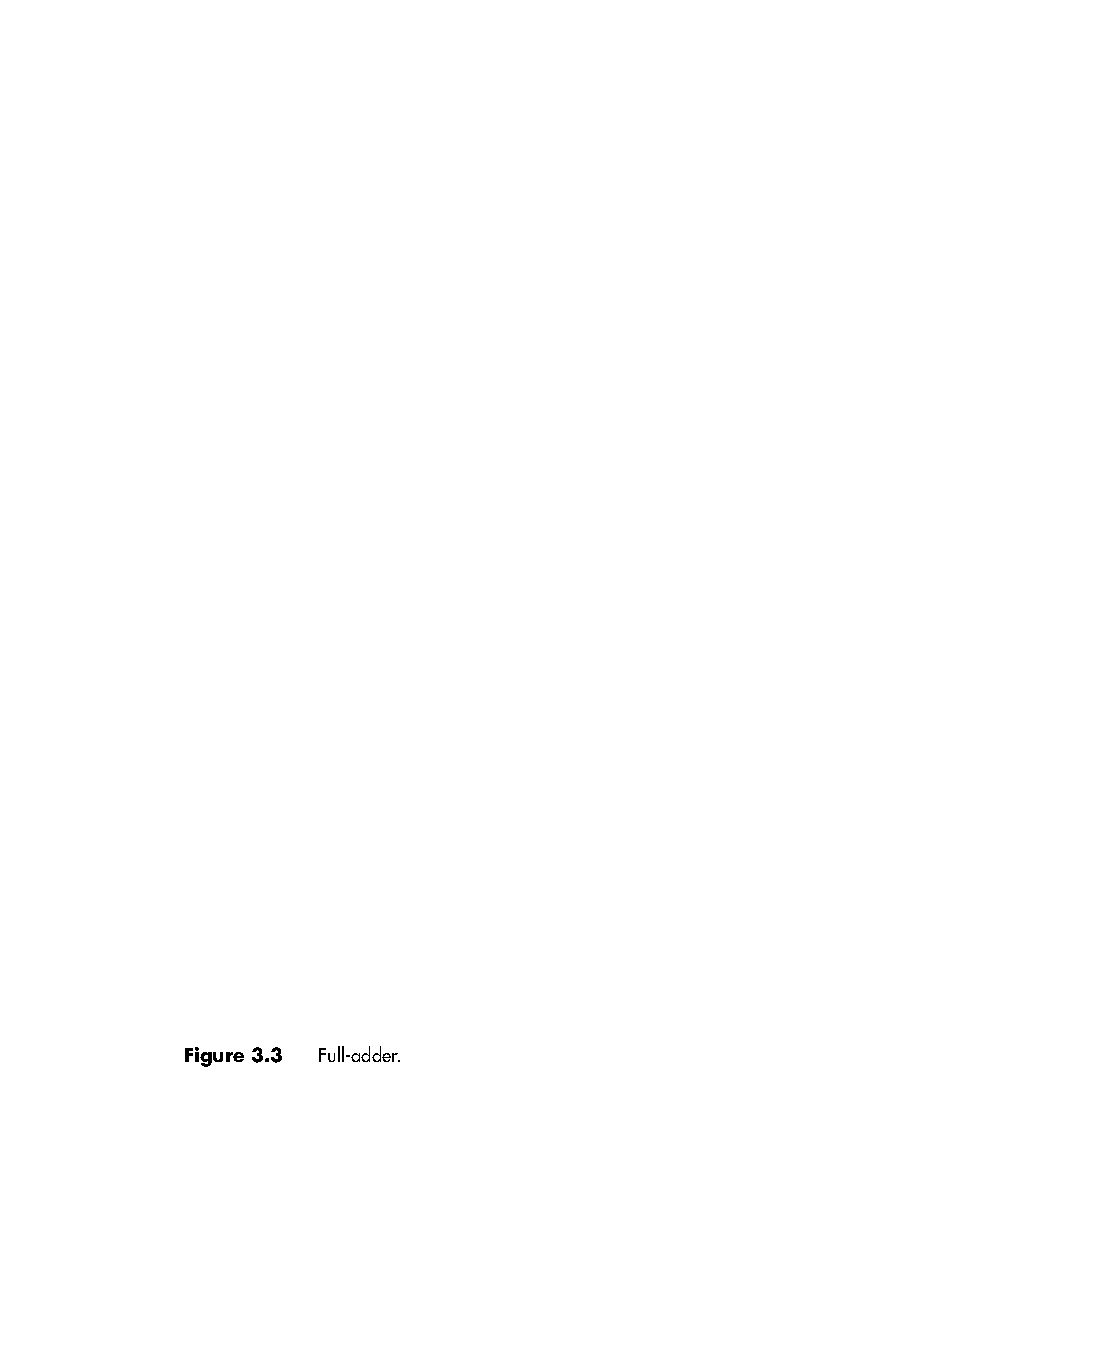
\includegraphics[]{VerilogFig3_3}
        \end{column}
    \end{columns}
\end{frame}

\begin{frame}{\insertsection} \center
    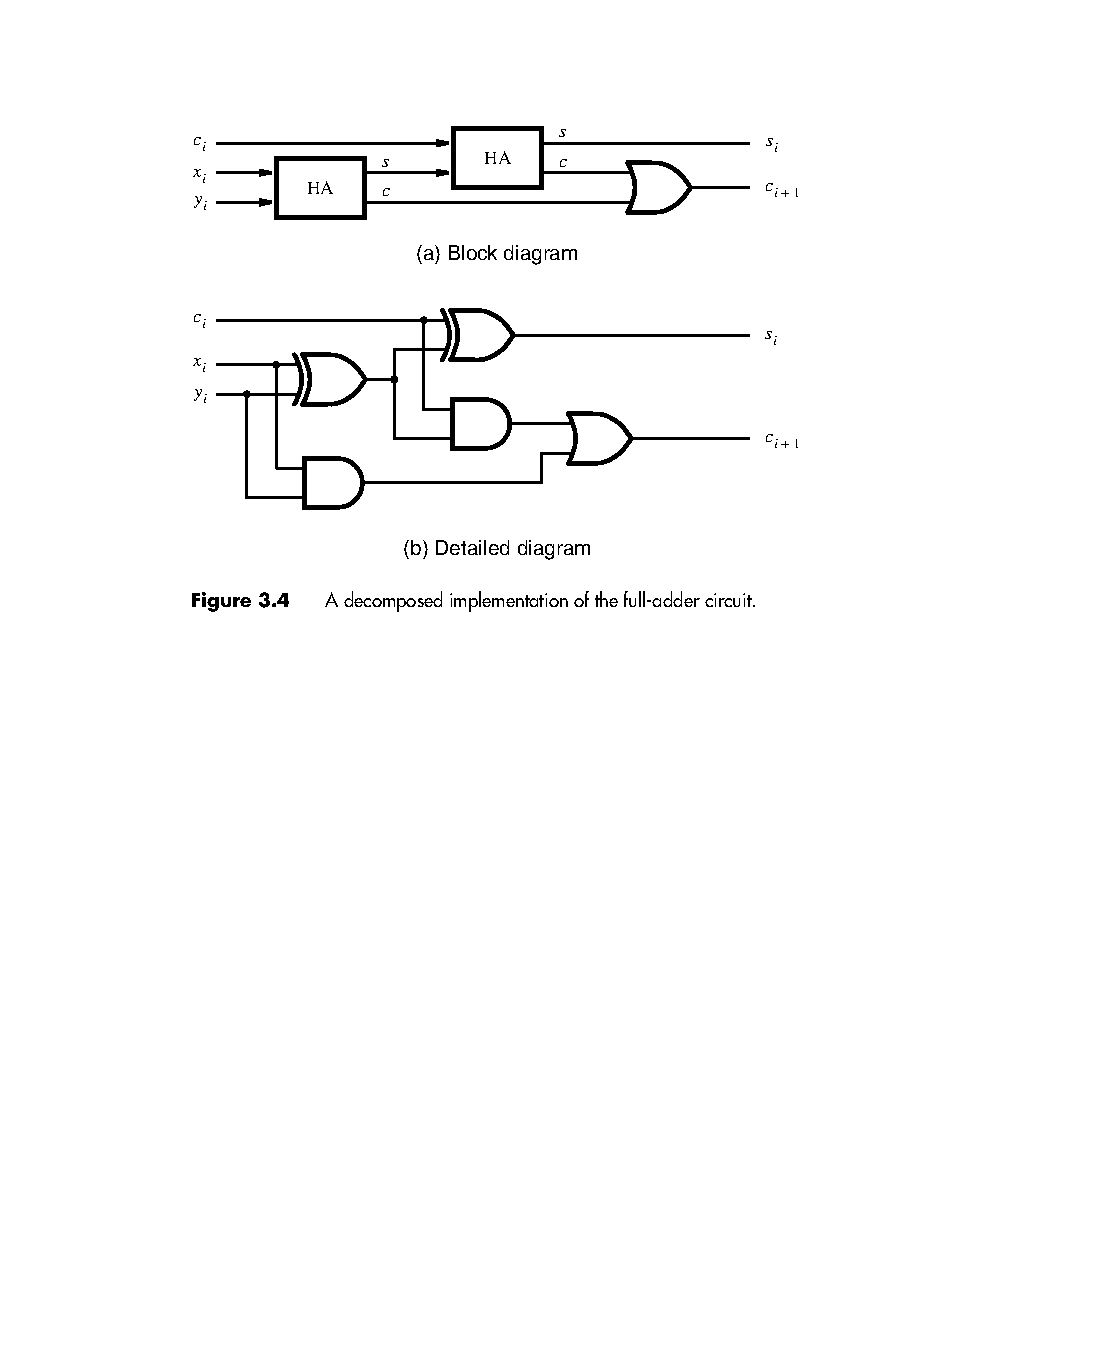
\includegraphics[width=.65\textwidth]{VerilogFig3_4}
\end{frame}

\begin{frame}{\insertsection} \center
    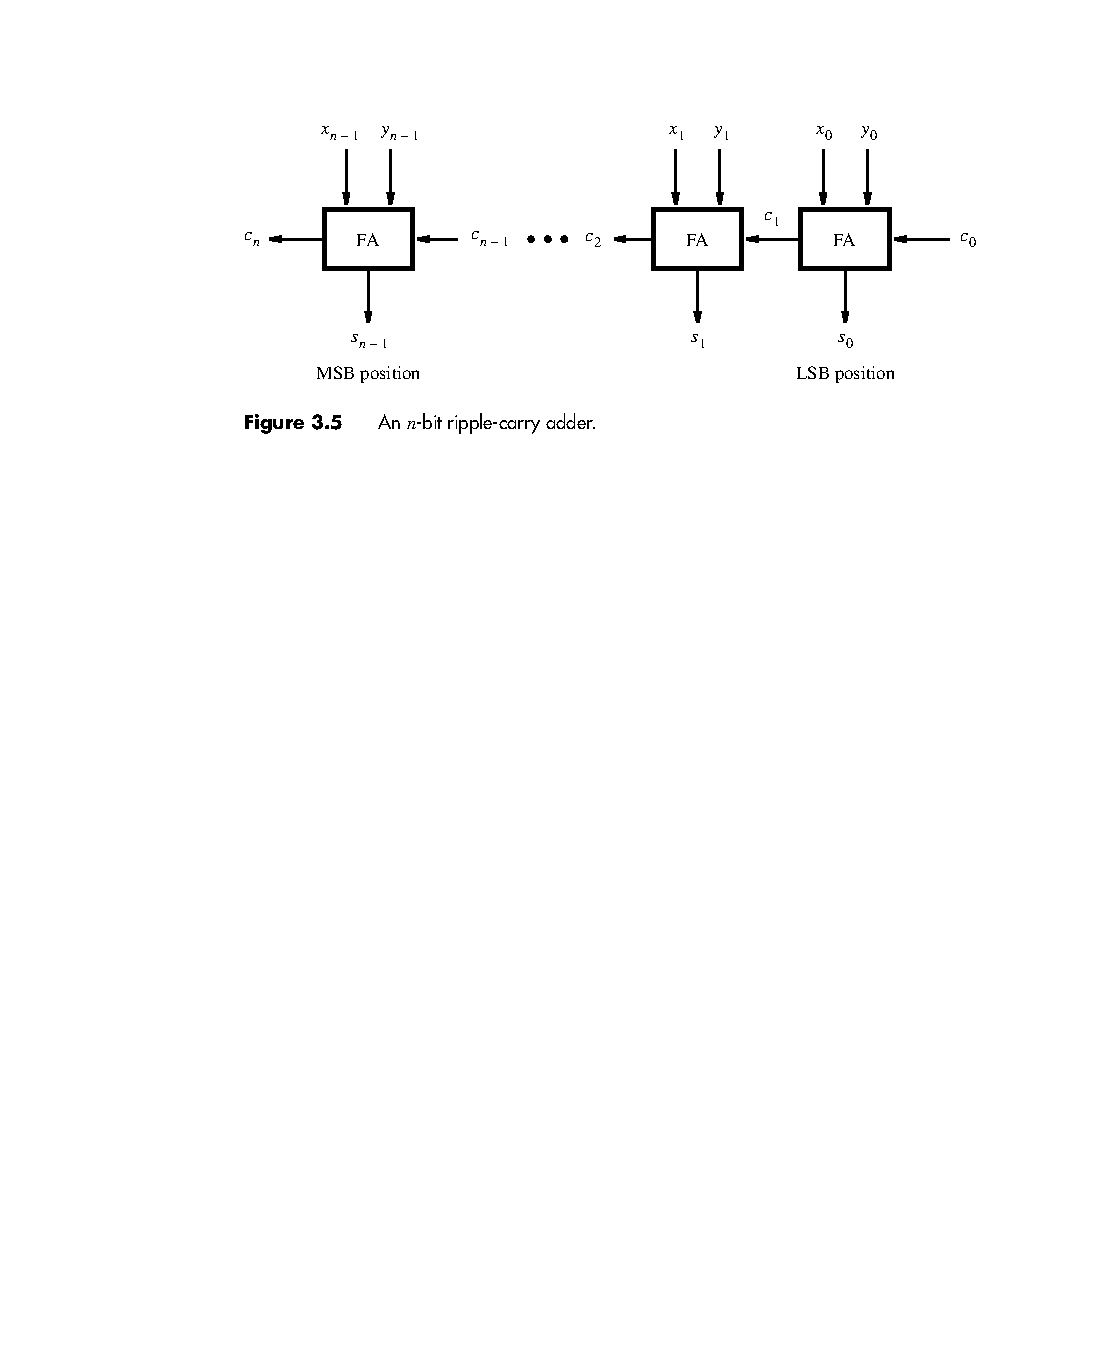
\includegraphics[width=\textwidth]{VerilogFig3_5}
\end{frame}

\begin{frame}{\insertsection} \center
    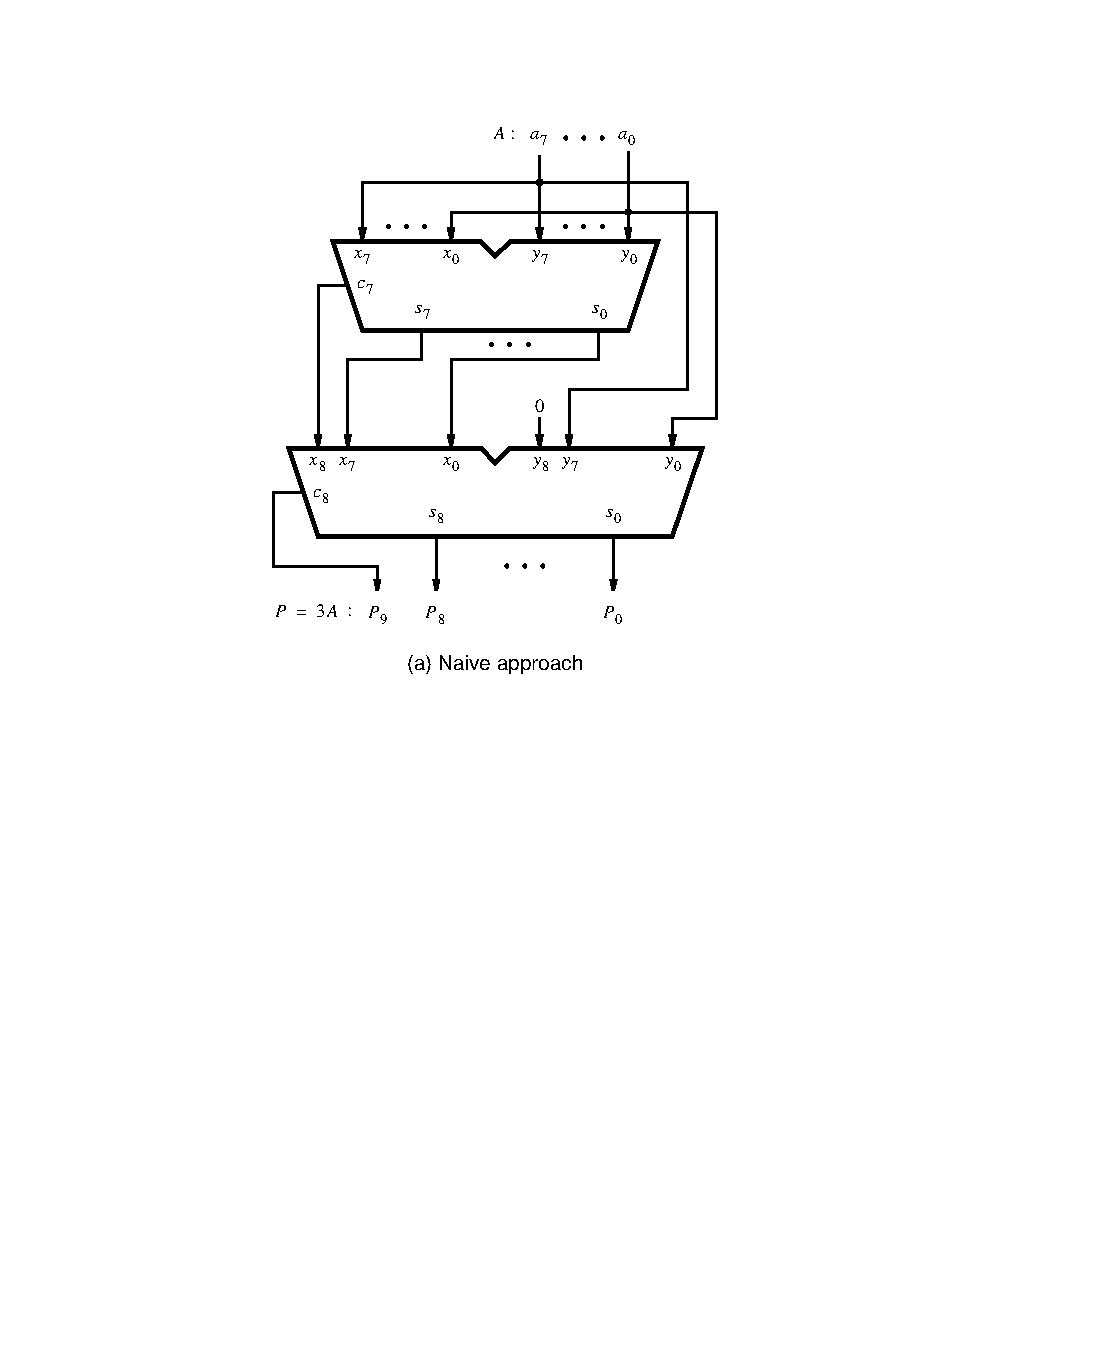
\includegraphics[width=.4\textwidth]{VerilogFig3_6a}
    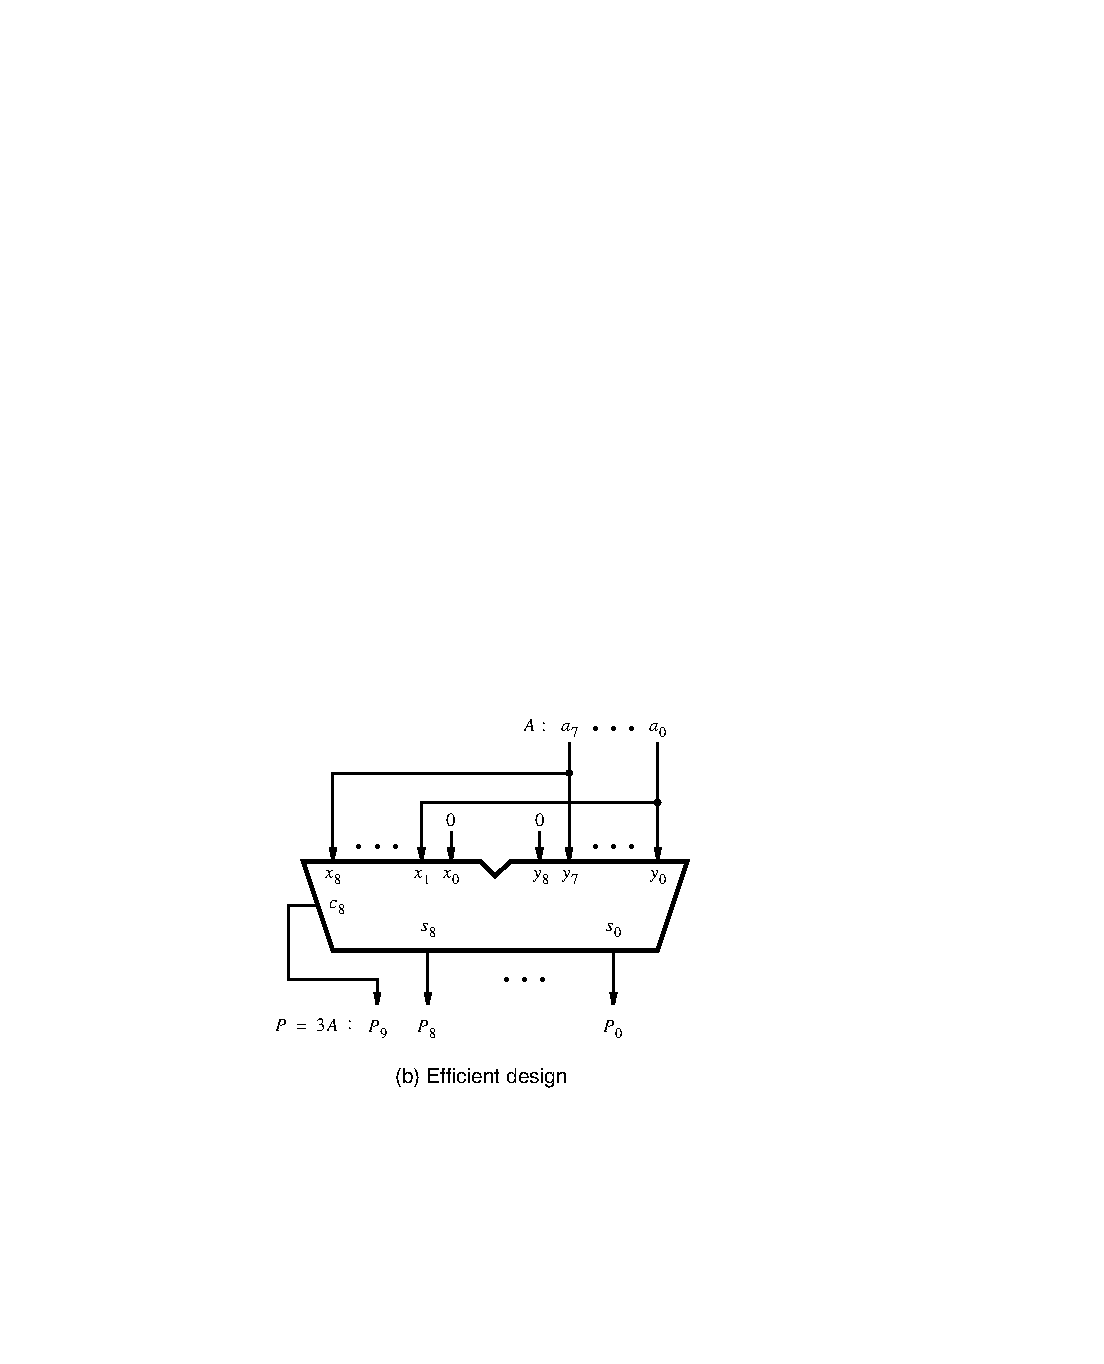
\includegraphics[width=.4\textwidth]{VerilogFig3_6b} \\
    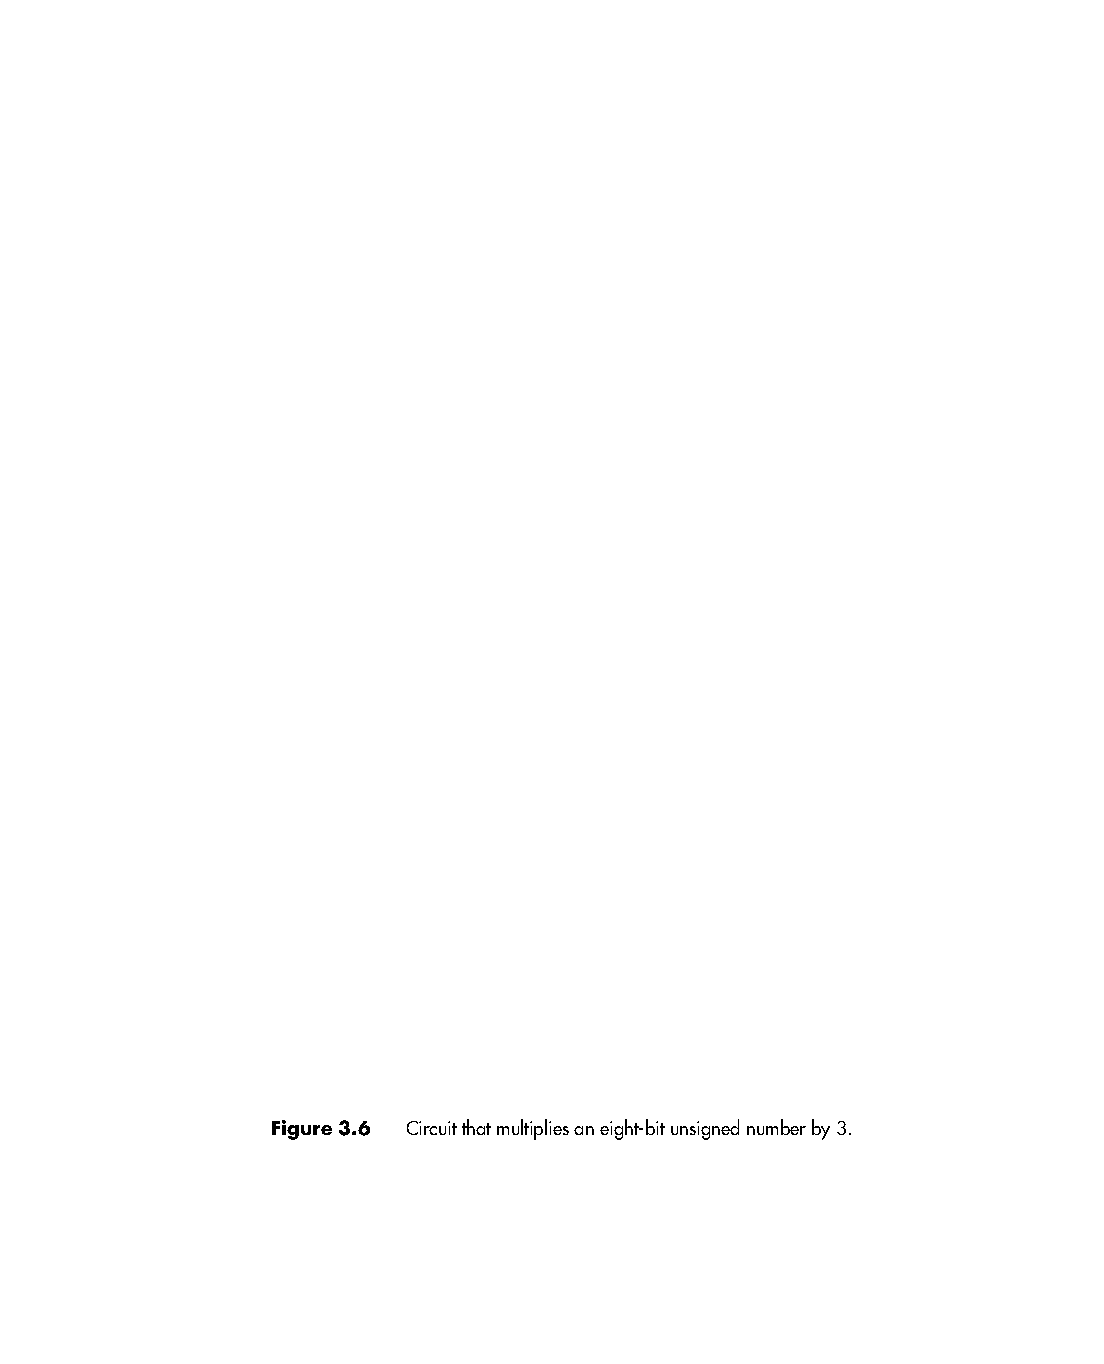
\includegraphics[width=.5\textwidth]{VerilogFig3_6}
\end{frame}

\section{Números com sinal}

\begin{frame}{\insertsection} \center
    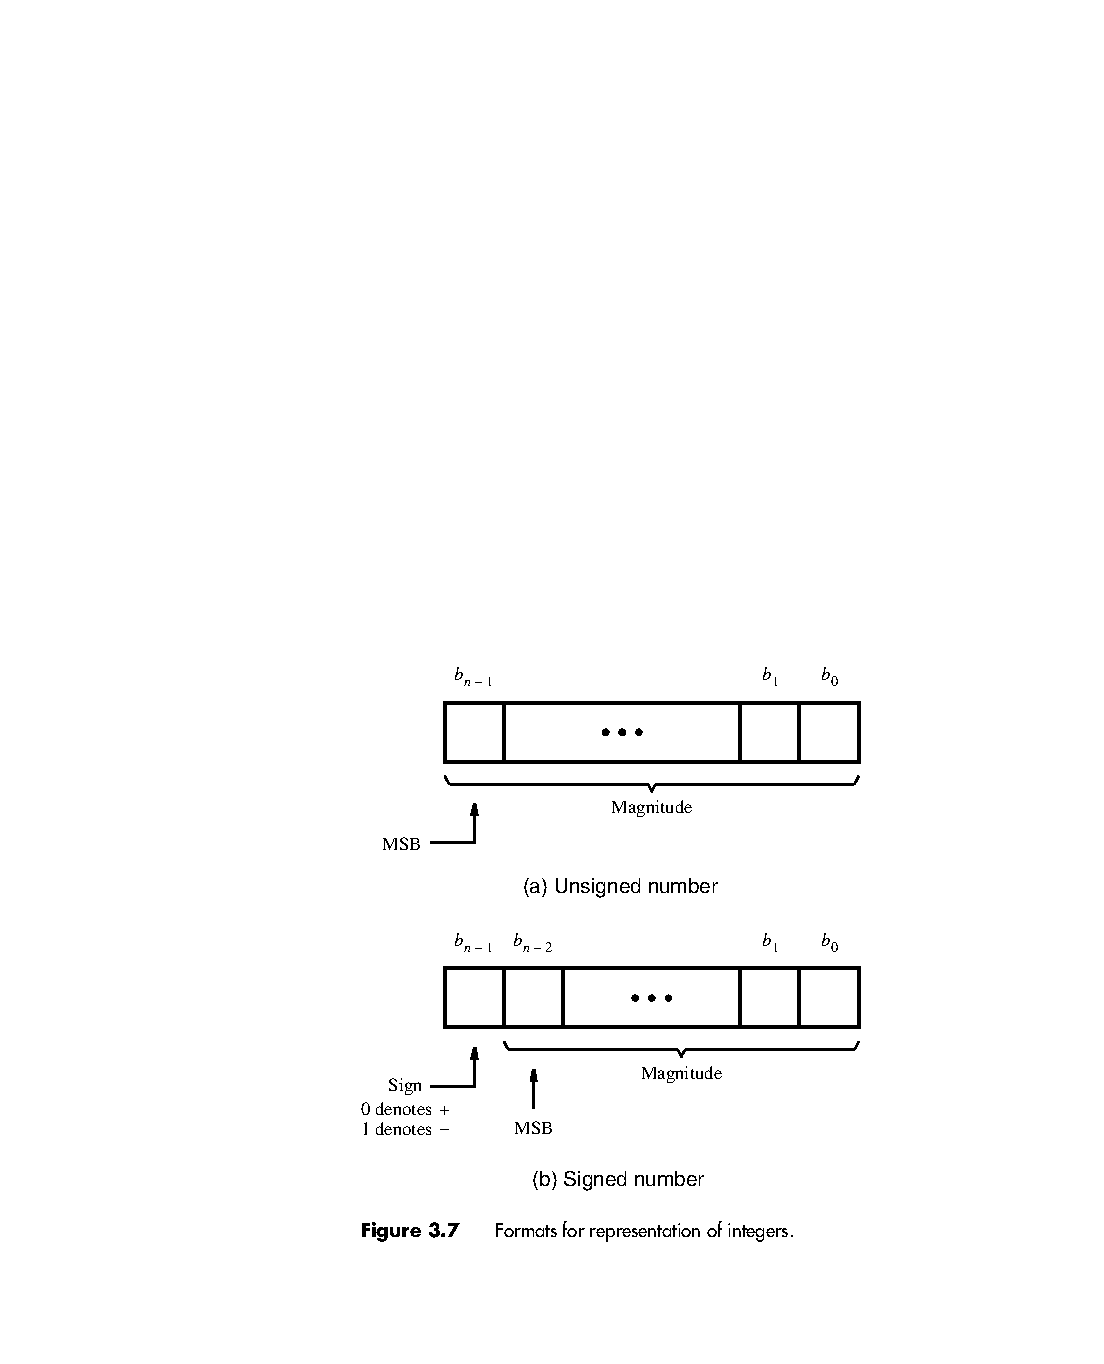
\includegraphics[width=.5\textwidth]{VerilogFig3_7}
\end{frame}

\begin{frame}{\insertsection} 
    \begin{itemize}
        \item Sinal/Magnitude 
        \begin{itemize}
            \item $+5 = 0101$ e $-5 = 1101$
        \end{itemize}
        \pause
        \item Complemento de 1 
        \begin{itemize}
            \item $K = (2^n - 1) - P$
            \item $+5 = 0101$ e $-5 = 1010$
        \end{itemize}
        \pause
        \item Complemento de 2
        \begin{itemize}
            \item $K = (2^n - P)$
            \item $+5 = 0101$ e $-5 = 1011$
            \item {\tt 0101~~~~~10110100~~~~~00000001~~~~~1000}
            \item {\tt 101\textbf{1}~~~~~01001\textbf{100}~~~~~1111111\textbf{1}~~~~~\textbf{1000!}}
        \end{itemize}
    \end{itemize}
\end{frame}

\begin{frame}{\insertsection} \center
    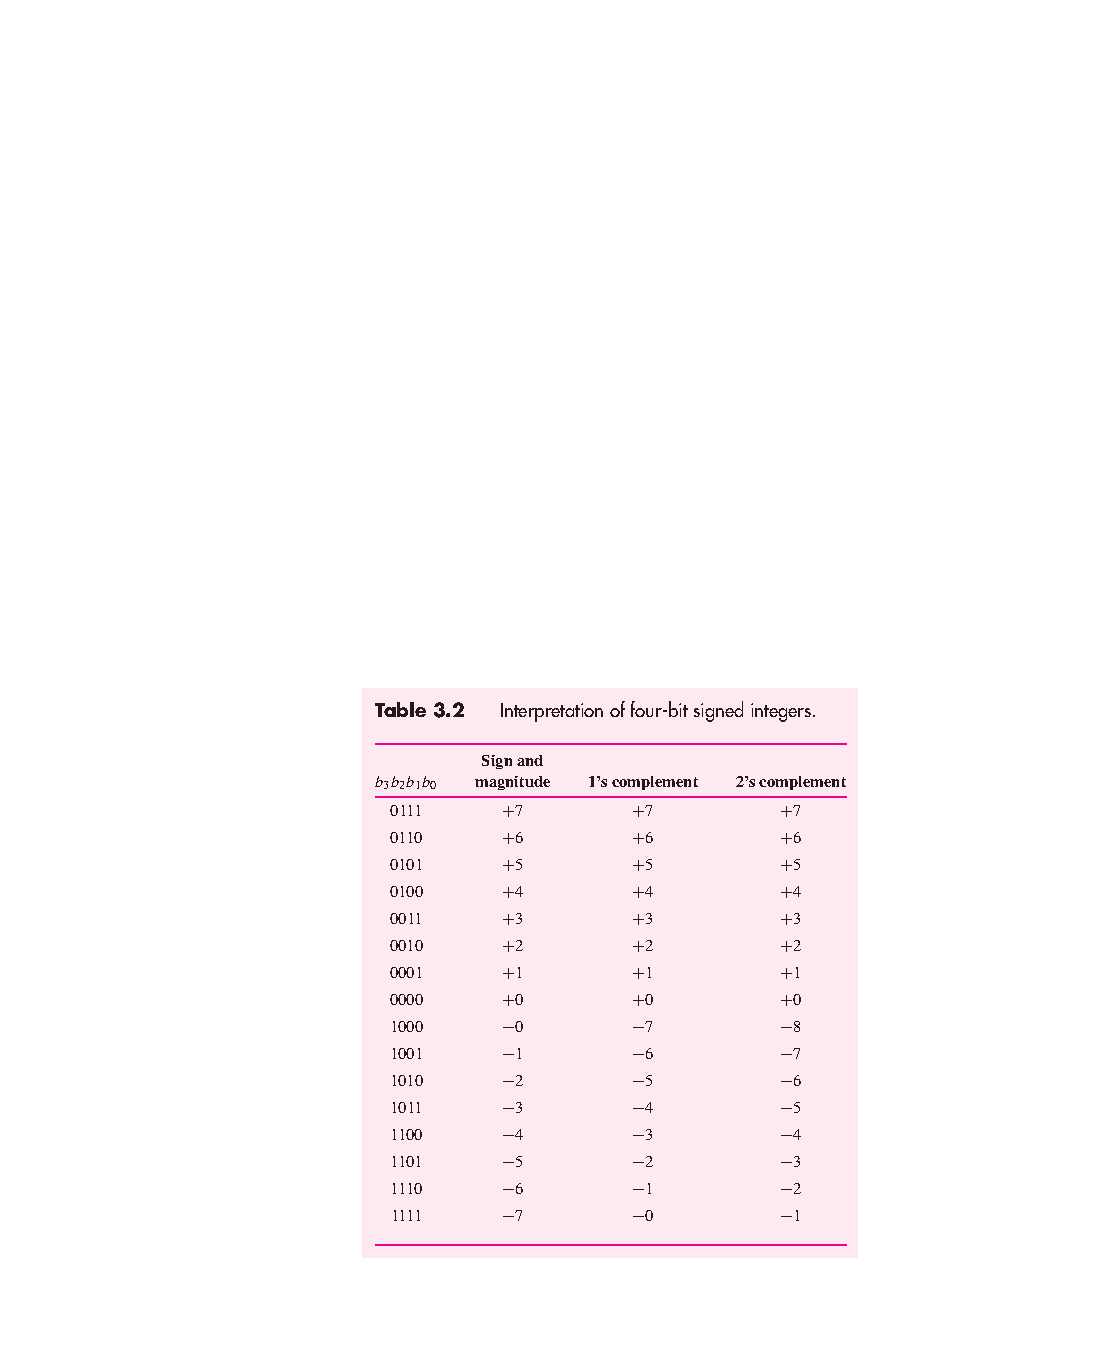
\includegraphics[width=.45\textwidth]{VerilogTab3_2}
\end{frame}

\begin{frame}{\insertsection} \center
    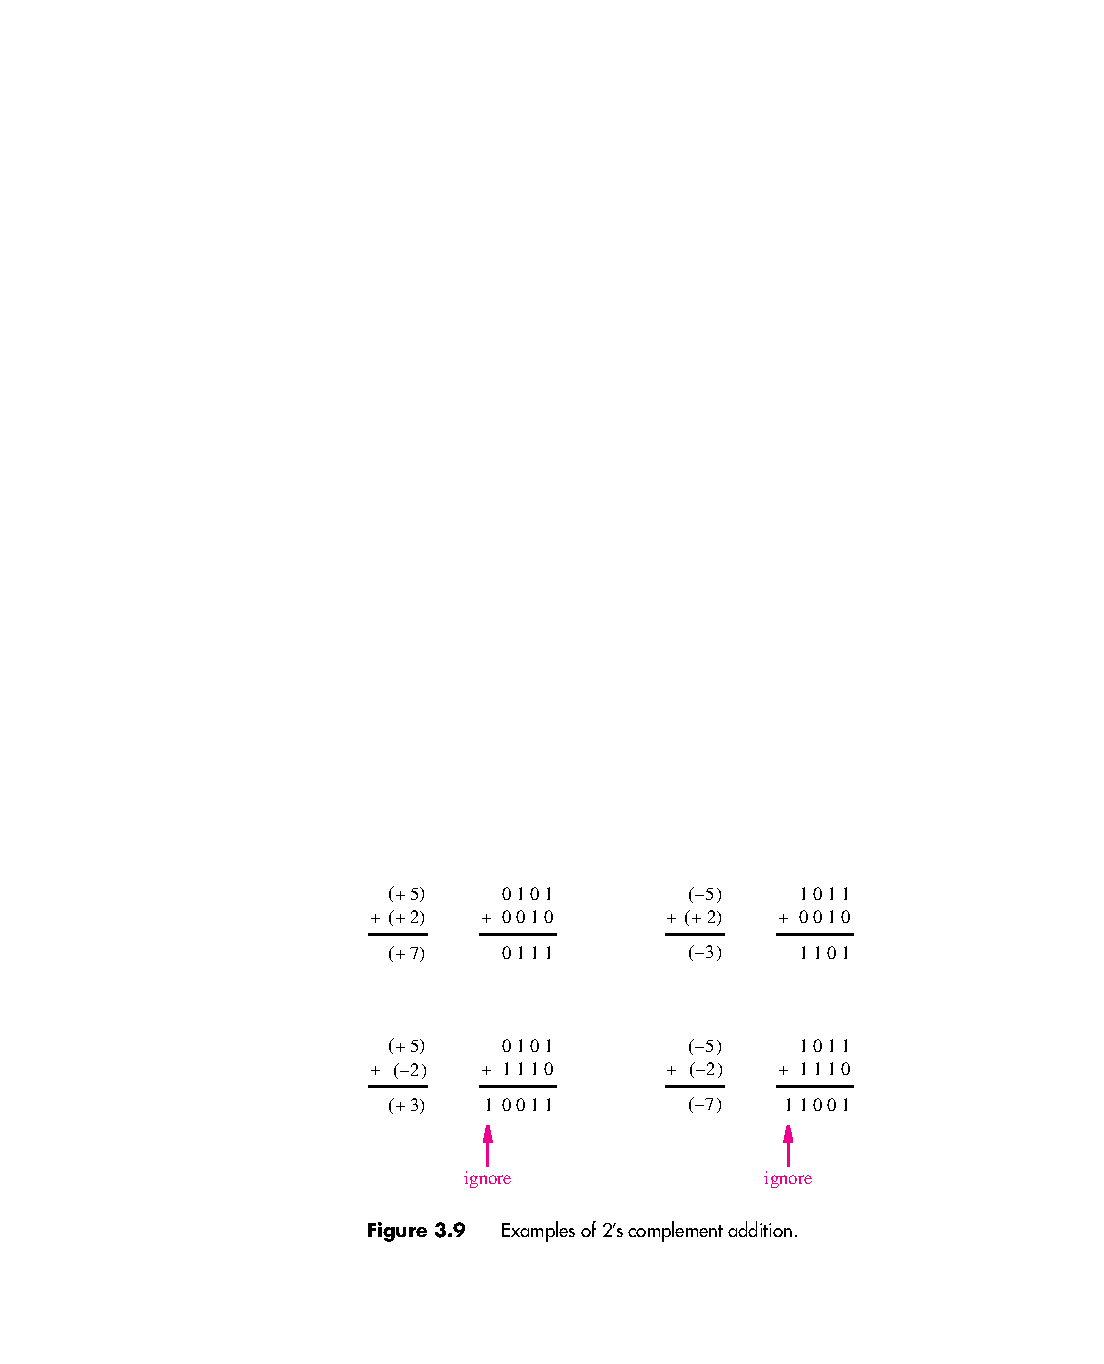
\includegraphics[width=.75\textwidth]{VerilogFig3_9}
\end{frame}

\begin{frame}{\insertsection} \center
    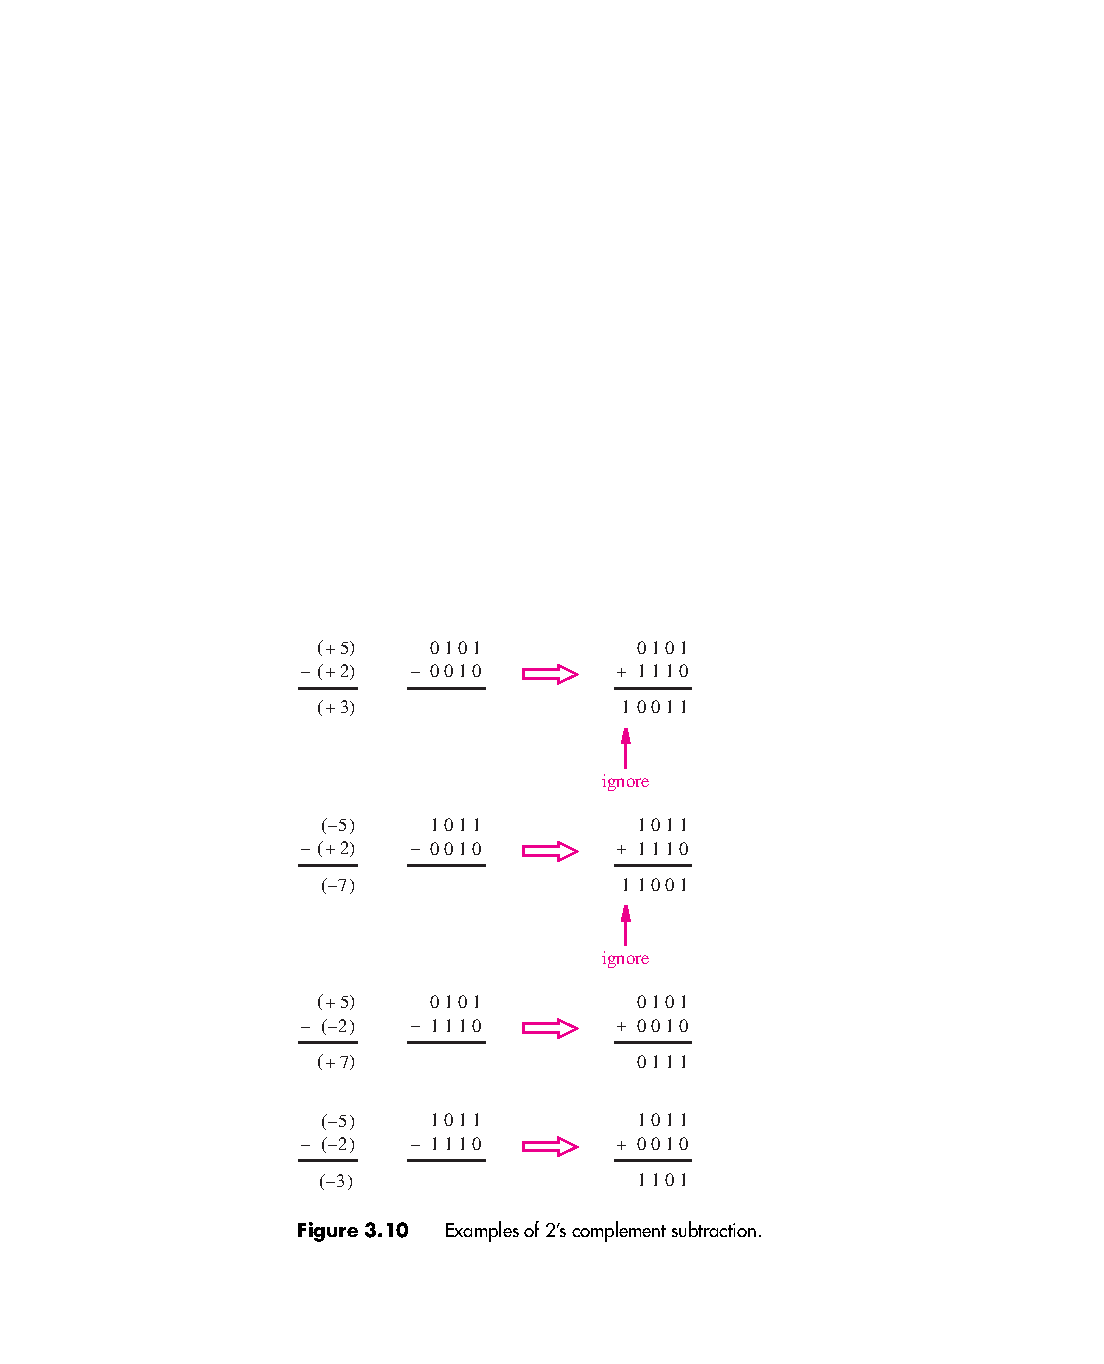
\includegraphics[width=.43\textwidth]{VerilogFig3_10}
\end{frame}

\begin{frame}{\insertsection} \center
    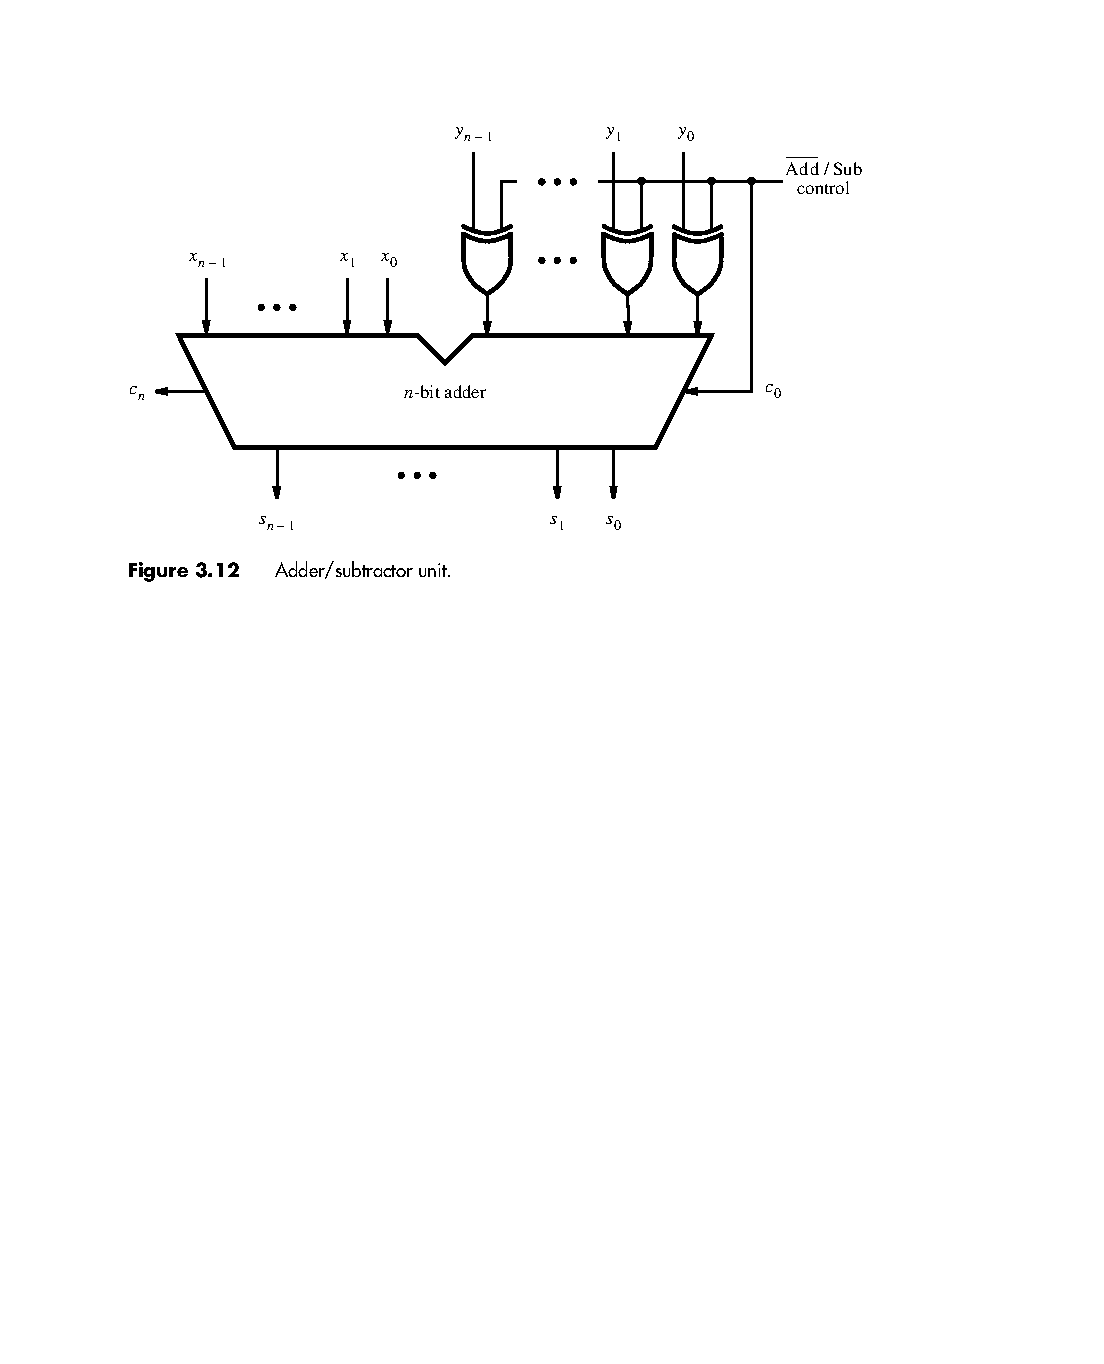
\includegraphics[width=.85\textwidth]{VerilogFig3_12}
\end{frame}

\begin{frame}{\insertsection} \center
    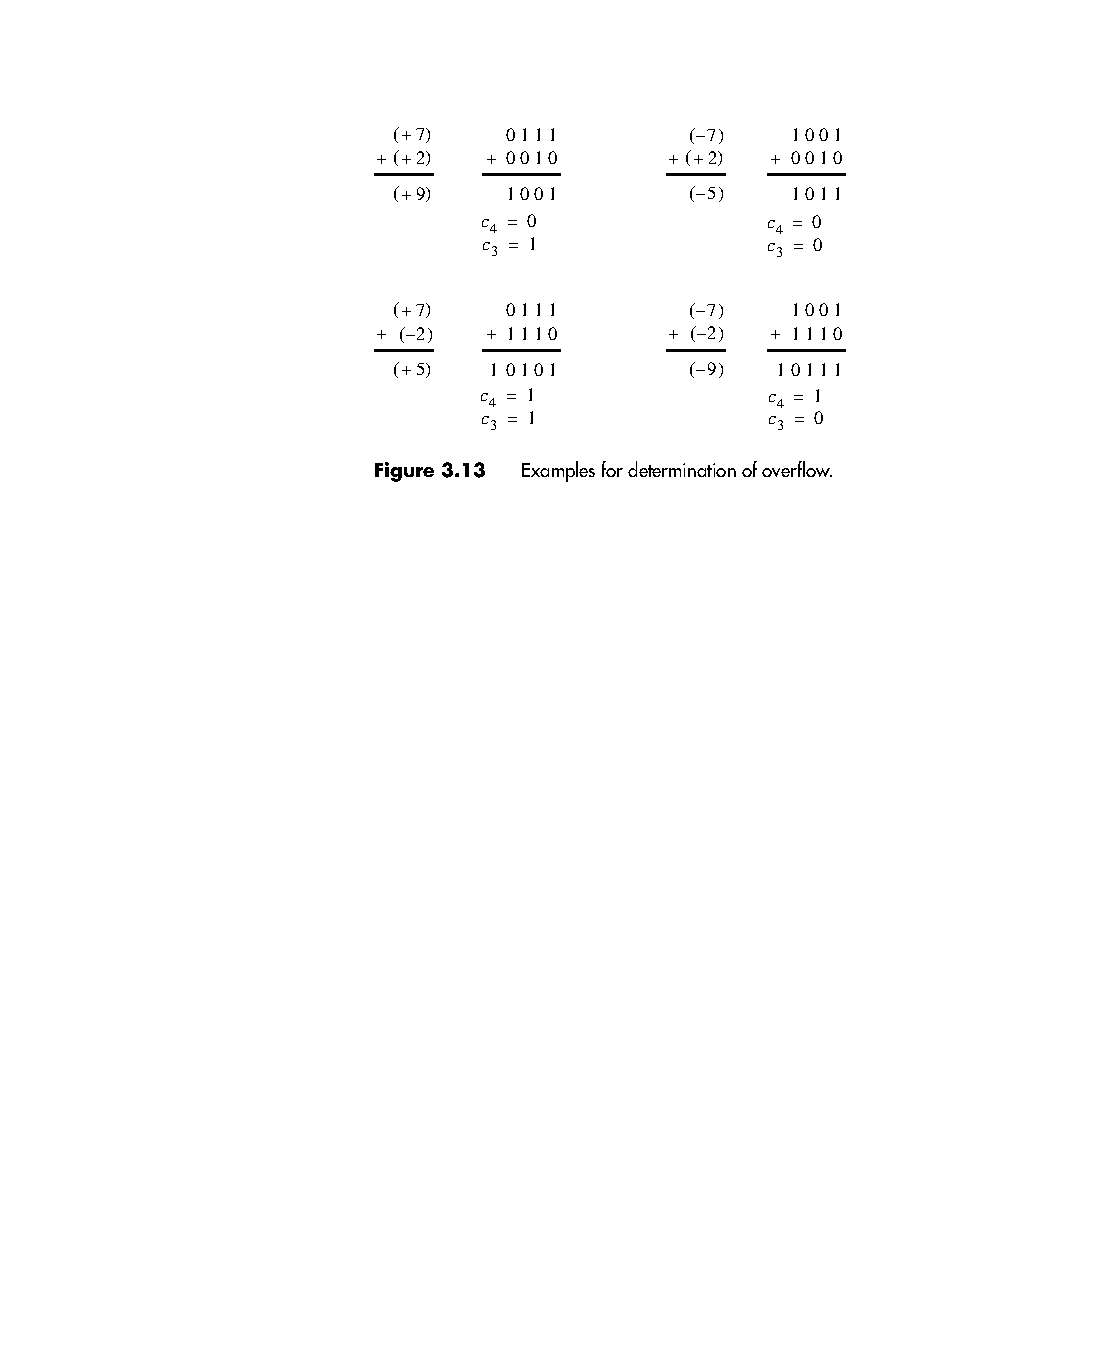
\includegraphics[width=.7\textwidth]{VerilogFig3_13}
\end{frame}

\begin{frame}{\insertsection} \center
    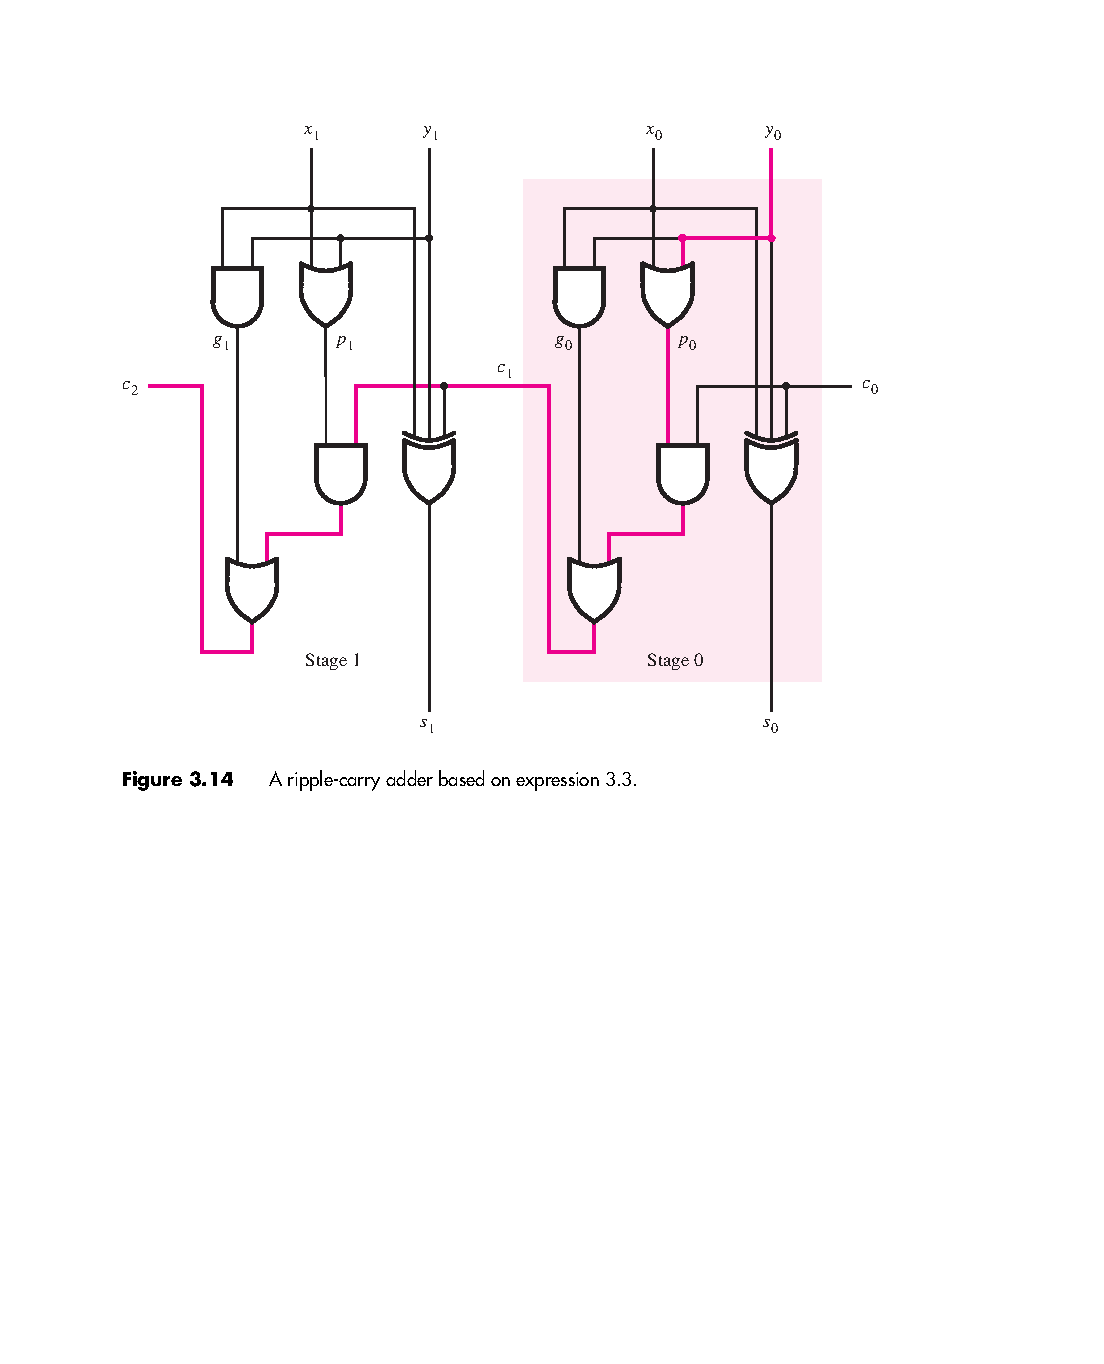
\includegraphics[width=.6\textwidth]{VerilogFig3_14}
\end{frame}

\begin{frame}{\insertsection} \center
    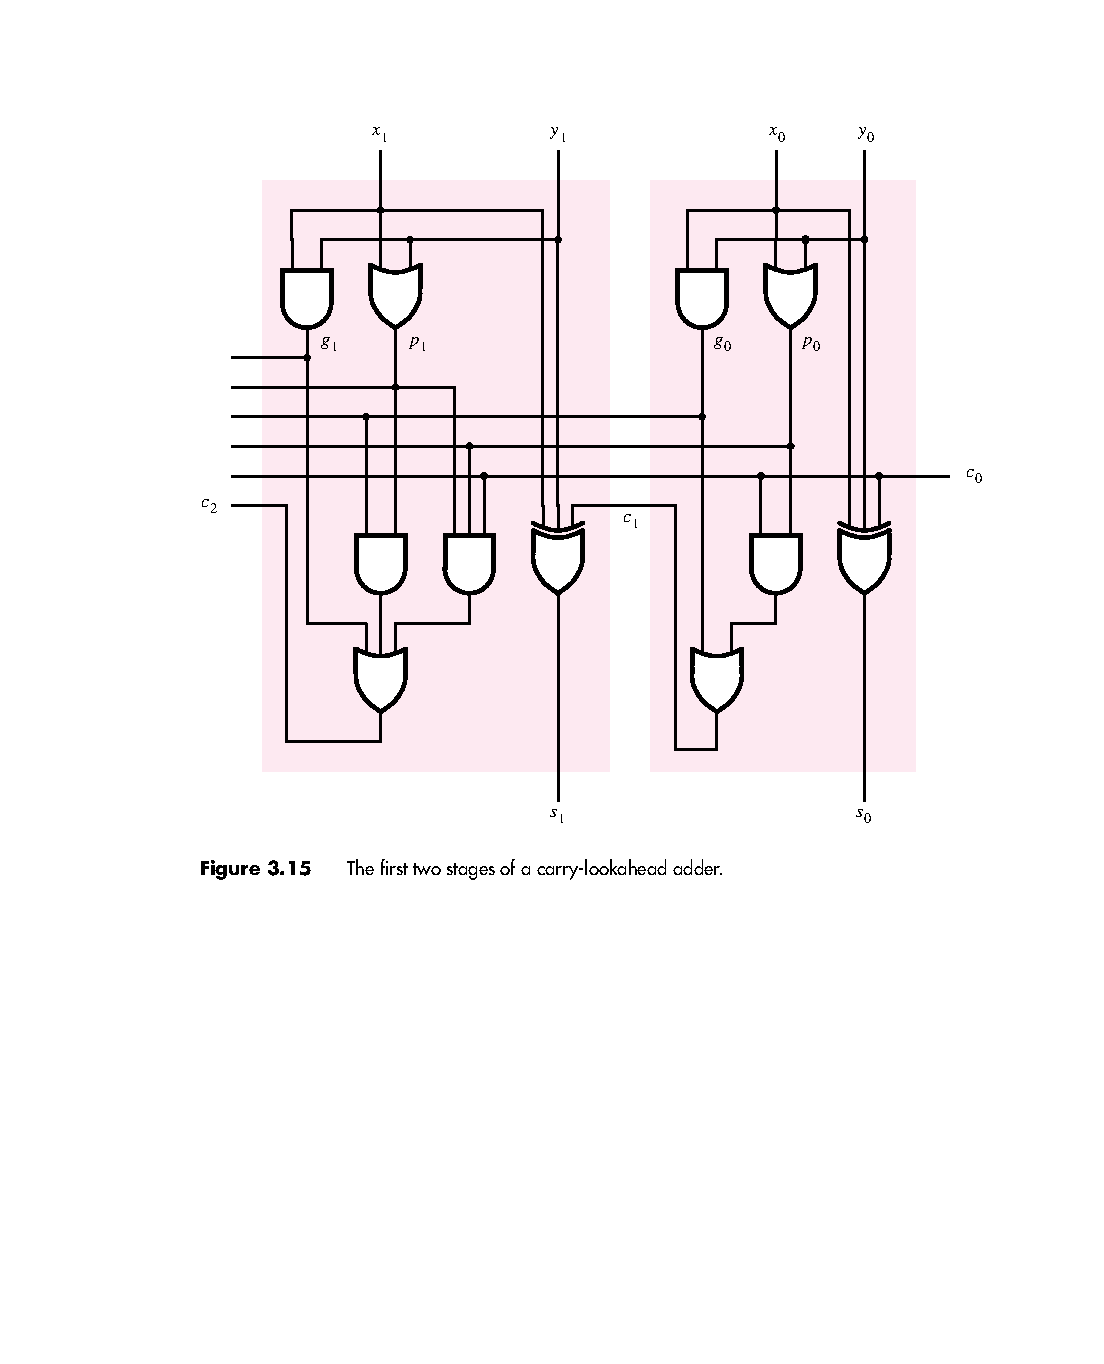
\includegraphics[width=.55\textwidth]{VerilogFig3_15}
\end{frame}

\section{Bibliografia} %%%%%%%

\begin{frame}{\insertsection} 
	\begin{itemize}
		\item \href{https://www.google.com.br/search?q=filetype\%3Apdf+Fundamentals+of+Digital+Logic+with+Verilog+Design+&oq=filetype\%3Apdf}{Brown, S. \& Vranesic, Z. - Fundamentals of Digital Logic with Verilog Design, 3rd Ed., Mc Graw Hill, 2009}
	\end{itemize}
\end{frame}

\begin{frame}
	\titlepage
\end{frame} 

\end{document}